\documentclass[a4paper,10pt]{article}

\usepackage{cite}
\usepackage{graphicx,color}
\usepackage{fancyhdr}
\usepackage{amstext,amsmath,amssymb}
\usepackage[shortlabels]{enumitem}

\usepackage{subcaption}
\usepackage{mwe}

\setlength{\oddsidemargin}{0cm} %
\setlength{\evensidemargin}{0cm} %
\setlength{\topmargin}{0cm} %
\setlength{\textwidth}{16cm} %
\setlength{\textheight}{22.5cm} %

\pagestyle{empty}
\newcommand{\assunto}{PARAFAC and Tensor Rank}

\sloppy
\definecolor{lightgray}{gray}{0.5}
\setlength{\parindent}{0pt}

\begin{document}

\thispagestyle{empty}

\begin{center}
  
    
\includegraphics[scale=0.10]{figs/icon.png}
    
    \LARGE{Universidade Federal do Ceará}
    
    \LARGE{Centro de Tecnologia}
    
    \LARGE{Departamento de Engenharia de Teleinformática}
    
    \LARGE{Engenharia de Teleinformática}
    
    \vspace{180pt}
      
    \LARGE{Multilinear Algebra}
      
    \LARGE{Computational Homeworks}
      
    \vspace{100pt}
    
\end{center}

\vspace{25pt}

\begin{flushleft}
	\begin{tabbing}
		Student \qquad Kenneth Brenner dos Anjos Benício – 519189\\
	   \qquad\qquad\qquad\= \\
		Professor\> Andre Lima Ferrer de Almeida \\
		Course \> Multilinear Algebra - TIP8419\\
	\end{tabbing}
\end{flushleft}

\vspace{25pt}

\begin{center}
    Fortaleza, 2022
\end{center}
\thispagestyle{empty}

\newpage

\thispagestyle{empty}

\newpage
\section*{Homework 0 \\ Kronecker Product Run Time}

    \subsection*{Run Time Perfomance of Sequential Kronecker Products}

    In here I will briefly analyze the run time performance of the inverse operator while also using the Kronecker Product. In the first case the number of products is fixed while the number of columns is varying. 
    In the second case we have a varying number of products for a fixed number of columns. In both cases is possible to see that is preferable to first invert the matrices before applying the Kronecker operator.  
    
    \begin{figure}[ht!]
        \centering 
        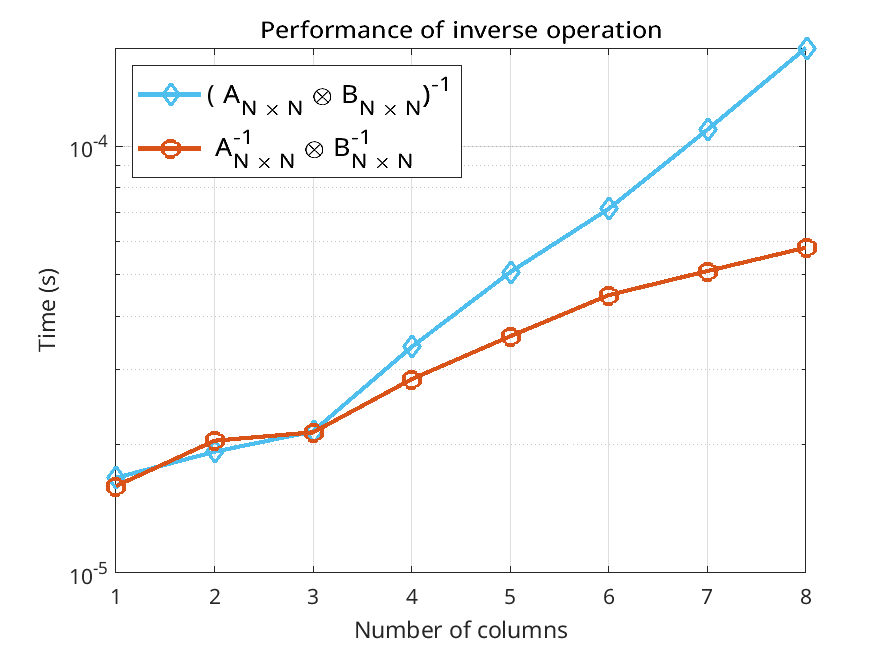
\includegraphics[width=0.65\linewidth]{figs/hw0a1.png} \par 
        \caption{Monter Carlo Experiment with 5000.}
        \label{fig:hw0a1} 
    \end{figure}

    \begin{figure}[ht!]
        \centering 
        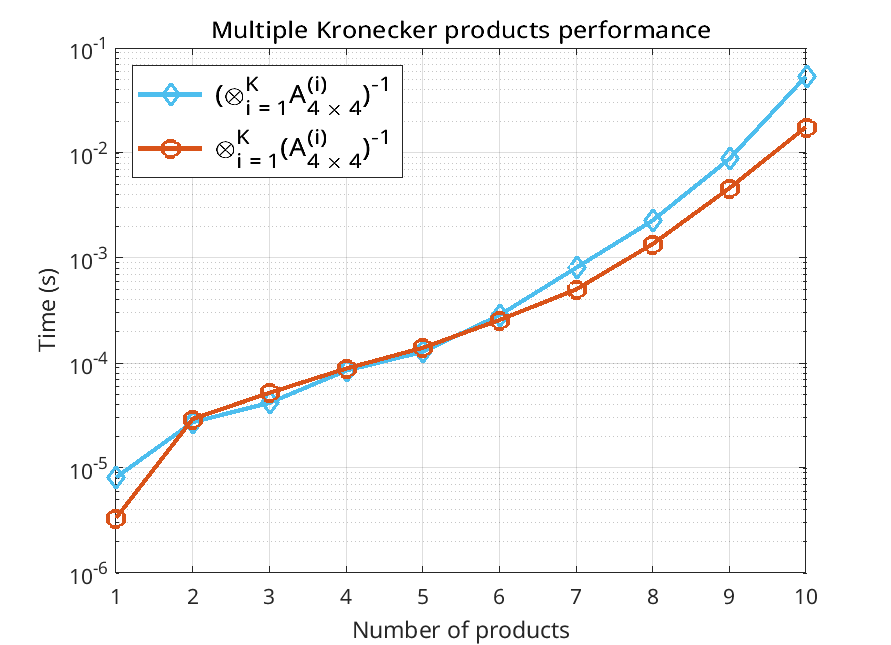
\includegraphics[width=0.65\linewidth]{figs/hw0a2.png} \par 
        \caption{Monter Carlo Experiment with 10000 runs.}
        \label{fig:hw0a2} 
    \end{figure}

    \newpage
    \subsection*{Show that $\text{eig}(\boldsymbol{A} \otimes \boldsymbol{B}) = \text{eig}(\boldsymbol{A}) \otimes \text{eig}(\boldsymbol{B})$}

    By using the eigenvalue decomposition (eig) of two matrices and apply the Kronecker Product to them it is possible to reach the intended result

    \begin{align}
        \boldsymbol{A} \otimes \boldsymbol{B} &= (\boldsymbol{C}_{1} \boldsymbol{\Lambda_{1}} \boldsymbol{C}^{-1}_{1}) \otimes (\boldsymbol{C}_{2} \boldsymbol{\Lambda_{2}} \boldsymbol{C}^{-1}_{2}), \\
        \boldsymbol{A} \otimes \boldsymbol{B} &= (\boldsymbol{C}_{1} \boldsymbol{\Lambda_{1}} \otimes \boldsymbol{C}_{2} \boldsymbol{\Lambda_{2}}) (\boldsymbol{C}^{-1}_{2} \otimes \boldsymbol{C}^{-1}_{2}), \\
        \boldsymbol{A} \otimes \boldsymbol{B} &= (\boldsymbol{C}_{1} \otimes \boldsymbol{C}_{2}) (\boldsymbol{\Lambda_{1}} \otimes \boldsymbol{\Lambda_{2}}) (\boldsymbol{C}^{-1}_{2} \otimes \boldsymbol{C}^{-1}_{2}), \\
        \text{eig}(\boldsymbol{A} \otimes \boldsymbol{B}) &= (\boldsymbol{\Lambda_{1}} \otimes \boldsymbol{\Lambda_{2}}) = \text{eig}(\boldsymbol{A}) \otimes \text{eig}(\boldsymbol{B}) 
    \end{align}

    \subsection*{Produced Algorithm}

    \begin{verbatim}
        %% ----- Homework 0 ----- %%
        clc;
        clear;
        close all;
        N = [1 2 3 4 5 6 7 8];
        time1 = zeros(length(N),1);
        time2 = zeros(length(N),1);
        for nn = 1:length(N)
            for mc = 1:5000
                A = randn(N(nn),N(nn)) + 1j*randn(N(nn),N(nn));
                B = randn(N(nn),N(nn)) + 1j*randn(N(nn),N(nn));
                tic;
                inv(tensor.mtx_prod_kron(A,B));
                aux = toc;
                time1(nn,1) = time1(nn,1) + aux;
                tic;
                tensor.mtx_prod_kron(inv(A),inv(B));
                aux = toc;
                time2(nn,1) = time2(nn,1) + aux;
            end
        end
        time1 = time1/5000;
        time2 = time2/5000;
        figure
        txt = ['(\bf A_{N \times N} \otimes B_{N \times N})^{-1}'];
        semilogy(N,time1,'-d','color', [0.3010 0.7450 0.9330], "linewidth", 2,...
            "markersize", 8, "DisplayName", txt);
        hold on;
        txt = ['\bf A^{-1}_{N \times N} \otimes B^{-1}_{N \times N}'];
        semilogy(N,time2,'-o','color', [0.8500 0.3250 0.0980], "linewidth", 2,...
            "markersize", 8, "DisplayName", txt);
        hold off;
        title(['Performance of inverse operation'])
        xlabel('Number of columns')
        ylabel('Time (s)')
        legend_copy = legend("location", "northwest");
        set(legend_copy,'Interpreter','tex','location','northwest',"fontsize", 12)
        grid on;
        saveas(gcf,'hw0a1.png')
        N = 2;
        K = [1 2 3 4 5 6 7 8 9 10];
        time1 = zeros(length(K),1);
        time2 = zeros(length(K),1);
        for kk = 1:length(K)
            for mc = 1:1000
                tic;
                for ii = 1:K(kk)    
                    if ii == 1
                        A1 = randn(N,N) + 1j*randn(N,N); 
                        continue
                    else
                        A2 = randn(N,N) + 1j*randn(N,N);
                        A1 = tensor.mtx_prod_kron(A1,A2);
                    end    
                end
                inv(A1);
                aux = toc;
                time1(kk,1) = time1(kk,1) + aux;
                
                tic;
                for ii = 1:K(kk)    
                    if ii == 1
                        A1 = randn(N,N) + 1j*randn(N,N); 
                        continue
                    else
                        A2 = randn(N,N) + 1j*randn(N,N);
                        A1 = tensor.mtx_prod_kron(inv(A1),inv(A2));
                    end    
                end
                aux = toc;
                time2(kk,1) = time2(kk,1) + aux;
            end
        end
        time1 = time1/1000;
        time2 = time2/1000;
        figure
        txt = ['\bf (\otimes^{K}_{i = 1}A^{(i)}_{4 \times 4})^{-1}'];
        semilogy(K,time1,'-d','color', [0.3010 0.7450 0.9330], "linewidth", 2,...
            "markersize", 8, "DisplayName", txt);
        hold on;
        txt = ['\bf \otimes^{K}_{i = 1}(A^{(i)}_{4 \times 4})^{-1}'];
        semilogy(K,time2,'-o','color', [0.8500 0.3250 0.0980], "linewidth", 2,...
            "markersize", 8, "DisplayName", txt);
        hold off;
        title(['Multiple Kronecker products performance'])
        xlabel('Number of products')
        ylabel('Time (s)')
        legend_copy = legend("location", "northwest");
        set(legend_copy,'Interpreter','tex','location','northwest',"fontsize", 12)
        grid on;
        saveas(gcf,'hw0a2.png')
    \end{verbatim}

\newpage
\section*{Homework 1 \\ Hadamard, Kronecker and Khatri-Rao Products}

    In Figure \ref{fig:hw1a1}, \ref{fig:hw1a2} and \ref{fig:hw1a3} I compare my implemention of Hadarmard, Kronecker and Khatri-Rao Products with the ones availables in the TensorLab package.
    As we can the only case where my function have shown an almost equal performance to the benchmark was the one where I do the Kronecker Product. The other two functions are far from the ideal
    performance offered by the TensorLab package. This could probably explained because I did not take full advantage of the vectorization that MATLAB offers when I was creating those two algorithms.

    \subsection*{Run Time Perfomance of Hadamard Product}

    \begin{figure}[ht!]
        \centering 
        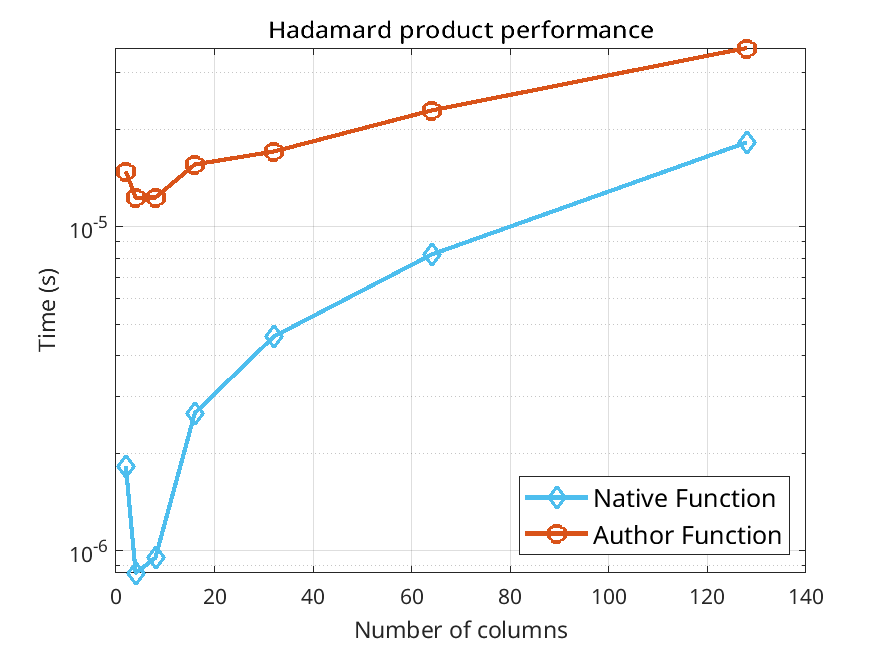
\includegraphics[width=0.65\linewidth]{figs/hw1a1.png} \par 
        \caption{Monter Carlo Experiment with 1000 runs.}
        \label{fig:hw1a1} 
    \end{figure}

    \subsection*{Run Time Perfomance of Kronecker Product}

    \begin{figure}[ht!]
        \centering 
        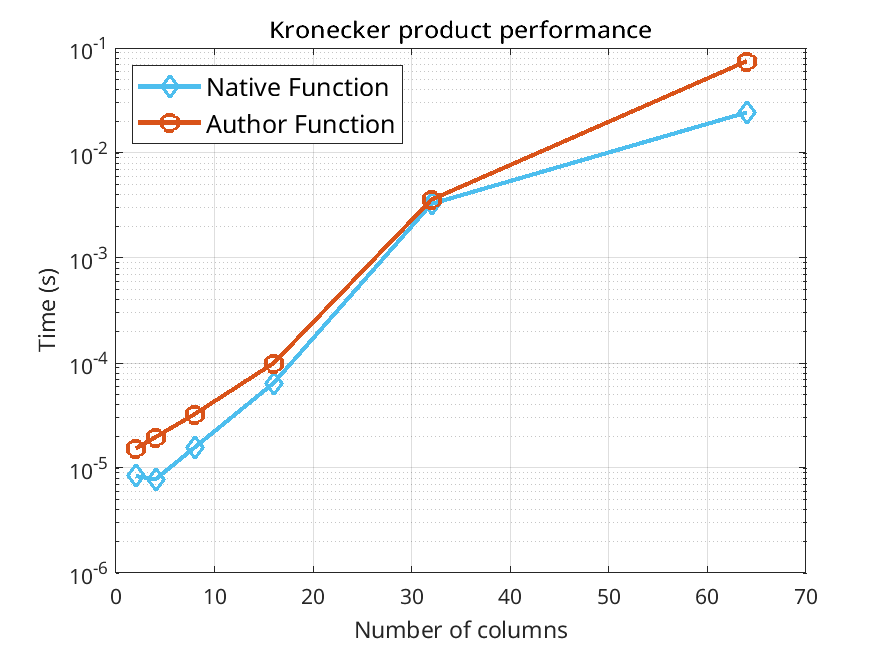
\includegraphics[width=0.65\linewidth]{figs/hw1a2.png} \par 
        \caption{Monter Carlo Experiment with 1000 runs.}
        \label{fig:hw1a2} 
    \end{figure}

    \subsection*{Run Time Perfomance of Khatri-Rao Product}

    \begin{figure}[ht!]
        \centering 
        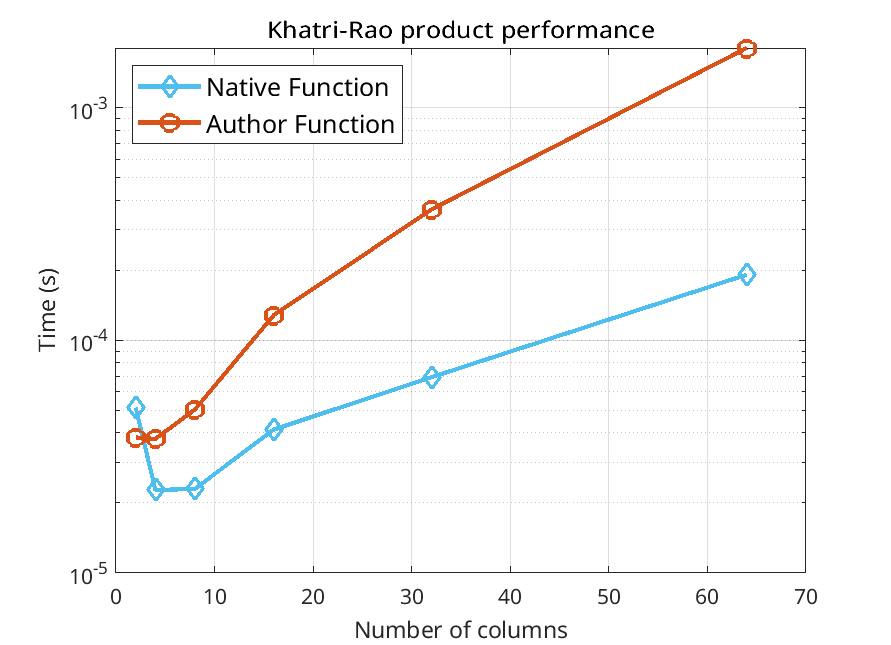
\includegraphics[width=0.65\linewidth]{figs/hw1a3.png} \par 
        \caption{Monter Carlo Experiment with 1000 runs.}
        \label{fig:hw1a3} 
    \end{figure}

    \newpage
    \subsection*{Produced Algorithm}

    \begin{verbatim}
        %% Hadamard Product

        % This function computes the Hadarmard Product of two given matrices.   
        % Author: Kenneth B. dos A. Benicio <kenneth@gtel.ufc.br>
        % Created: January 2022

        function C = mtx_prod_had(A,B)
            
            [ia,ja] = size(A);
            [ib,jb] = size(B);
            
            if (ia ~= ib) || (ja~=jb)
                disp('Invalid Matrices!')
                return;
            else
                C = A.*B;
                %C = zeros(ia,ja);
                %for i = 1:ia 
                    %for j = 1:ja
                        %C(i,j) = A(i,j)*B(i,j);
                    %end
                %end
            end
        end

        %% Kronecker Product

        % This function computes the Kronecker Product of two given matrices. 
        % Author: Kenneth B. dos A. Benicio <kenneth@gtel.ufc.br>
        % Created: January 2022

        function C = mtx_prod_kron(A,B)
            
            [ia,ja] = size(A);
            [ib,jb] = size(B);
            
            A = repelem(A,ib,jb);
            B = repmat(B,[ia ja]);
            C = A.*B;
            
        end

        %% Khatri-Rao Product

        % This function computes the Khatri-Rao Product of two given matrices. 
        % Author: Kenneth B. dos A. Benicio <kenneth@gtel.ufc.br>
        % Created: January 2022

        function C = mtx_prod_kr(A,B)
            [ia,ja] = size(A);
            [ib,jb] = size(B);
            
            if (ja~=jb)
                disp('Invalid Matrices!')
                return;
            else
                C = zeros(ia*ib,ja);
                for j = 1:ja
                    C(:,j) = tensor.mtx_prod_kron(A(:,j),B(:,j));
                end
            end
        end

        %% ----- Homework 1 ----- %%
        clc;
        clear;
        close all;
        
        N = [2 4 8 16 32 64 128];
        time1 = zeros(length(N),1);
        time2 = zeros(length(N),1);
        for nn = 1:length(N)
            for mc = 1:1000
                A = randn(N(nn),N(nn)) + 1j*randn(N(nn),N(nn));
                B = randn(N(nn),N(nn)) + 1j*randn(N(nn),N(nn));
                tic;
                A.*B;
                aux = toc;
                time1(nn,1) = time1(nn,1) + aux;
                tic;
                tensor.mtx_prod_had(A,B);
                aux = toc;
                time2(nn,1) = time2(nn,1) + aux;
            end
        end
        time1 = time1/1000;
        time2 = time2/1000;

        figure
        txt = ['Native Function'];
        semilogy(N,time1,'-d','color', [0.3010 0.7450 0.9330], "linewidth", 2,...
            "markersize", 8, "DisplayName", txt);
        hold on;
        txt = ['Author Function'];
        semilogy(N,time2,'-o','color', [0.8500 0.3250 0.0980], "linewidth", 2,...
            "markersize", 8, "DisplayName", txt);
        hold off;
        title(['Hadamard product performance'])
        xlabel('Number of columns')
        ylabel('Time (s)')
        legend_copy = legend("location", "southeast");
        set(legend_copy,'Interpreter','tex','location','southeast',"fontsize", 12)
        grid on;
        saveas(gcf,'hw1a1.png')

        N = [2 4 8 16 32 64];
        time1 = zeros(length(N),1);
        time2 = zeros(length(N),1);
        for nn = 1:length(N)
            for mc = 1:1000
                A = randn(N(nn),N(nn)) + 1j*randn(N(nn),N(nn));
                B = randn(N(nn),N(nn)) + 1j*randn(N(nn),N(nn));
                tic;
                kron(A,B);
                aux = toc;
                time1(nn,1) = time1(nn,1) + aux;
                tic;
                tensor.mtx_prod_kron(A,B);
                aux = toc;
                time2(nn,1) = time2(nn,1) + aux;
            end
        end
        time1 = time1/1000;
        time2 = time2/1000;

        figure
        txt = ['Native Function'];
        semilogy(N,time1,'-d','color', [0.3010 0.7450 0.9330], "linewidth", 2,...
            "markersize", 8, "DisplayName", txt);
        hold on;
        txt = ['Author Function'];
        semilogy(N,time2,'-o','color', [0.8500 0.3250 0.0980], "linewidth", 2,...
            "markersize", 8, "DisplayName", txt);
        hold off;
        title(['Kronecker product performance'])
        xlabel('Number of columns')
        ylabel('Time (s)')
        legend_copy = legend("location", "northwest");
        set(legend_copy,'Interpreter','tex','location','northwest',"fontsize", 12)
        grid on;
        saveas(gcf,'hw1a2.png')

        N = [2 4 8 16 32 64];
        time1 = zeros(length(N),1);
        time2 = zeros(length(N),1);
        for nn = 1:length(N)
            for mc = 1:1000
                A = randn(N(nn),N(nn)) + 1j*randn(N(nn),N(nn));
                B = randn(N(nn),N(nn)) + 1j*randn(N(nn),N(nn));
                tic;
                kr(A,B);
                aux = toc;
                time1(nn,1) = time1(nn,1) + aux;
                tic;
                tensor.mtx_prod_kr(A,B);
                aux = toc;
                time2(nn,1) = time2(nn,1) + aux;
            end
        end
        time1 = time1/1000;
        time2 = time2/1000;

        figure
        txt = ['Native Function'];
        semilogy(N,time1,'-d','color', [0.3010 0.7450 0.9330], "linewidth", 2,...
            "markersize", 8, "DisplayName", txt);
        hold on;
        txt = ['Author Function'];
        semilogy(N,time2,'-o','color', [0.8500 0.3250 0.0980], "linewidth", 2,...
            "markersize", 8, "DisplayName", txt);
        hold off;
        title(['Khatri-Rao product performance'])
        xlabel('Number of columns')
        ylabel('Time (s)')
        legend_copy = legend("location", "northwest");
        set(legend_copy,'Interpreter','tex','location','northwest',"fontsize", 12)
        grid on;
        saveas(gcf,'hw1a3.png')
    \end{verbatim}

\newpage
\section*{Homework 2 \\ Khatri-Rao Product Run Time}

    \subsection*{Run Time Performance of Khatri-Rao Product for Different Implementations}

    In Figures \ref{fig:hw2a1} and \ref{fig:hw2a2} we can see the processing time for the considered methods to compute the pseudoinverse of a Khatri-Rao product for the cases
    where we have two and four columns in each matrix. To draw the curves it was implemented a Monte Carlo Experiment with only 250 runs for each value $N$ of rows with $N \in \{2, 4, 8, 16, 32, 64\}$.
    For both cases we can see a clear advantage in using the third method as the dimmensions of the matrices increases. In a similar maner, we can also observe that the second method is a bit better than the first however 
    not as good as the third. To see a better behavior for these methods it should be necessary to increase the number of rows to better analyse the advantages of each one, however due to technical constraints 
    I could not increase as much as I wanted. In the sequence we can see the definition of each implemented method.

    \begin{align}
        (\boldsymbol{A} \diamond \boldsymbol{B})^{\dagger} &= \text{pinv}(\boldsymbol{A} \diamond \boldsymbol{B}), \\
        (\boldsymbol{A} \diamond \boldsymbol{B})^{\dagger} &= [(\boldsymbol{A} \diamond \boldsymbol{B})^{\text{T}} (\boldsymbol{A} \diamond \boldsymbol{B})]^{-1} (\boldsymbol{A} \diamond \boldsymbol{B})^{\text{T}}, \\
        (\boldsymbol{A} \diamond \boldsymbol{B})^{\dagger} &= [(\boldsymbol{A}^{\text{T}}\boldsymbol{A})(\boldsymbol{B}^{\text{T}}\boldsymbol{B})]^{-1} (\boldsymbol{A} \diamond \boldsymbol{B})^{\text{T}}, 
    \end{align}

    \begin{figure}[ht!]
        \centering 
        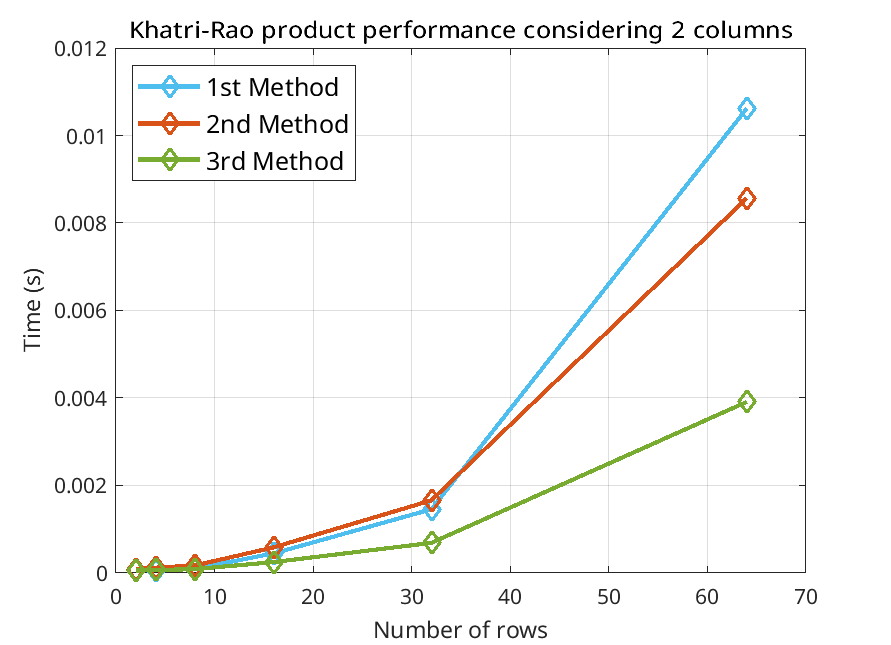
\includegraphics[width=0.75\linewidth]{figs/hw2a1.png} \par 
        \caption{Monter Carlo Experiment with 250 runs and R = 2.}
        \label{fig:hw2a1}
    \end{figure}

    \begin{figure}[ht!]
        \centering 
        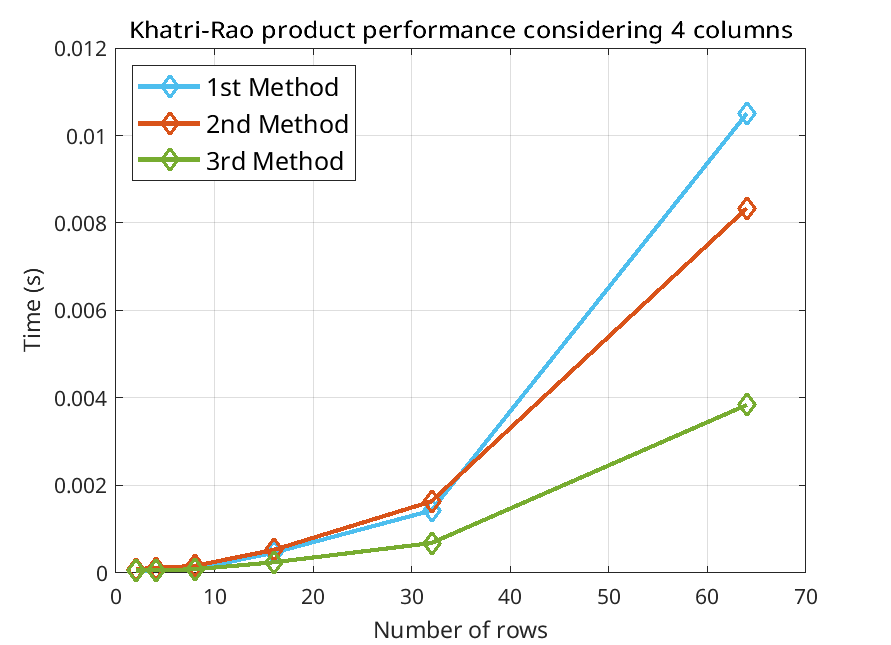
\includegraphics[width=0.75\linewidth]{figs/hw2a2.png} \par 
        \caption{Monter Carlo Experiment with 250 runs and R = 4.}
        \label{fig:hw2a2} 
    \end{figure}

    \subsection*{Run Time Perfomance of Sequential Khatri-Rao Products}

    In Figure \ref{fig:hw2a3} we analyze the behavior of the Khatri-Rao product when sequential products are taken. As we can see it is an exponencial curve since after every product we will have matrices with analyse
    increasing dimmensions. Thus, when we do need to use consecutive Khatri-Rao products we should seek a way to simplify the operation by using algebraic manipulations.

    \begin{figure}[ht!]
        \centering 
        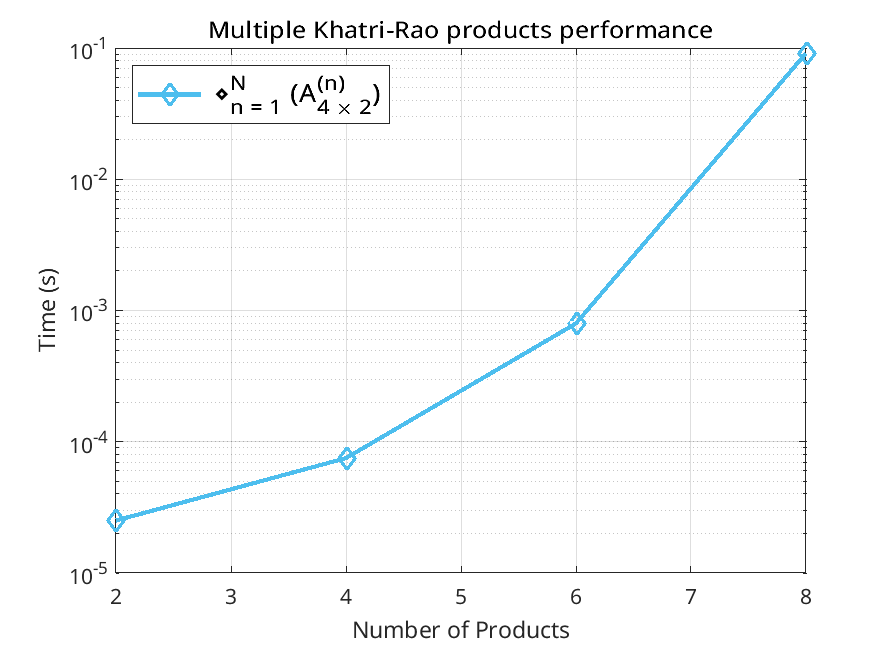
\includegraphics[width=0.75\linewidth]{figs/hw2a3.png} \par 
        \caption{Monter Carlo Experiment with 250 runs.}
        \label{fig:hw2a3} 
    \end{figure}
    
    \newpage
    \subsection*{Produced Algorithm}

    \begin{verbatim}
        %% ----- Homework 2 ----- %%
        clc;
        clear;
        close all;

        R = 2;
        I = [2 4 8 16 32 64];
        time1 = zeros(length(I),1);
        time2 = zeros(length(I),1);
        time3 = zeros(length(I),1);
        for ii = 1:length(I)
            for mc = 1:250
                A = randn(I(ii),I(ii)) + 1j*randn(I(ii),I(ii));
                B = randn(I(ii),I(ii)) + 1j*randn(I(ii),I(ii));
                tic;
                pinv(tensor.mtx_prod_kr(A,B));
                aux = toc;
                time1(ii,1) = time1(ii,1) + aux;
                tic;
                (tensor.mtx_prod_kr(A,B).'*tensor.mtx_prod_kr(A,B))...
                    \(tensor.mtx_prod_kr(A,B).');
                aux = toc;
                time2(ii,1) = time2(ii,1) + aux;
                tic;
                tensor.mtx_prod_had((A.'*A),(B.'*B))\(tensor.mtx_prod_kr(A,B).');
                aux = toc;
                time3(ii,1) = time3(ii,1) + aux;
            end
        end
        time1 = time1/250;
        time2 = time2/250;
        time3 = time3/250;

        figure
        txt = ['1st Method'];
        plot(I,time1,'-d','color', [0.3010 0.7450 0.9330], "linewidth", 2,...
            "markersize", 8, "DisplayName", txt);
        hold on;
        txt = ['2nd Method'];
        plot(I,time2,'-d','color', [0.8500 0.3250 0.0980], "linewidth", 2,...
            "markersize", 8, "DisplayName", txt);
        hold on;
        txt = ['3rd Method'];
        plot(I,time3,'-d','color', [0.4660 0.6740 0.1880], "linewidth", 2,...
            "markersize", 8, "DisplayName", txt);
        hold off;
        title(['Khatri-Rao product performance considering 2 columns'])
        xlabel('Number of rows')
        ylabel('Time (s)')
        legend_copy = legend("location", "northwest");
        set(legend_copy,'Interpreter','tex','location','northwest',"fontsize", 12)
        grid on;
        saveas(gcf,'hw2a1.png')

        R = 4;
        I = [2 4 8 16 32 64];
        time1 = zeros(length(I),1);
        time2 = zeros(length(I),1);
        time3 = zeros(length(I),1);
        for ii = 1:length(I)
            for mc = 1:250
                A = randn(I(ii),I(ii)) + 1j*randn(I(ii),I(ii));
                B = randn(I(ii),I(ii)) + 1j*randn(I(ii),I(ii));
                tic;
                pinv(tensor.mtx_prod_kr(A,B));
                aux = toc;
                time1(ii,1) = time1(ii,1) + aux;
                tic;
                (tensor.mtx_prod_kr(A,B).'*tensor.mtx_prod_kr(A,B))...
                    \(tensor.mtx_prod_kr(A,B).');
                aux = toc;
                time2(ii,1) = time2(ii,1) + aux;
                tic;
                tensor.mtx_prod_had((A.'*A),(B.'*B))\(tensor.mtx_prod_kr(A,B).');
                aux = toc;
                time3(ii,1) = time3(ii,1) + aux;
            end
        end
        time1 = time1/250;
        time2 = time2/250;
        time3 = time3/250;

        figure
        txt = ['1st Method'];
        plot(I,time1,'-d','color', [0.3010 0.7450 0.9330], "linewidth", 2,...
            "markersize", 8, "DisplayName", txt);
        hold on;
        txt = ['2nd Method'];
        plot(I,time2,'-d','color', [0.8500 0.3250 0.0980], "linewidth",...
            2, "markersize", 8, "DisplayName", txt);
        hold on;
        txt = ['3rd Method'];
        plot(I,time3,'-d','color', [0.4660 0.6740 0.1880], "linewidth",...
            2, "markersize", 8, "DisplayName", txt);
        hold off;
        title(['Khatri-Rao product performance considering 4 columns'])
        xlabel('Number of rows')
        ylabel('Time (s)')
        legend_copy = legend("location", "northwest");
        set(legend_copy,'Interpreter','tex','location','northwest',"fontsize", 12)
        grid on;
        saveas(gcf,'hw2a2.png')

        I = 4;
        R = 2;
        N = [2 4 6 8];
        time1 = zeros(length(N),1);
        time2 = zeros(length(N),1);
        for nn = 1:length(N)
            for mc = 1:250 
                tic;
                for ii = 1:N(nn)
                    if ii == 1
                        A1 = randn(I,R) + 1j*randn(I,R); 
                        continue
                    else
                        A2 = randn(I,R) + 1j*randn(I,R);
                        A1 = tensor.mtx_prod_kron(A1,A2);
                    end    
                end
                aux = toc;
                time1(nn,1) = time1(nn,1) + aux;
            end
        end
        time1 = time1/250;

        figure
        txt = ['\bf \diamond^{N}_{n = 1} (A^{(n)}_{4 \times 2})'];
        semilogy(N,time1,'-d','color', [0.3010 0.7450 0.9330], "linewidth", 2,...
            "markersize", 8, "DisplayName", txt);
        title(['Multiple Khatri-Rao products performance'])
        xlabel('Number of Products')
        ylabel('Time (s)')
        legend_copy = legend("location", "northwest");
        set(legend_copy,'Interpreter','tex','location','northwest',"fontsize", 12)
        grid on;
        saveas(gcf,'hw2a3.png')
    \end{verbatim}

\newpage
\section*{Homework 3 \\ Least-Squares Khatri-Rao Factorization (LSKRF)}

    \subsection*{Implementation LSKRF}

    The LSKRF algorithm aims to solve the following estimation problem 

    \begin{align}
        \left(\hat{\boldsymbol{A}}, \hat{\boldsymbol{B}}\right) = \underset{\boldsymbol{A}, \boldsymbol{B}}{\text{min}} \left|\left| \boldsymbol{X} - \boldsymbol{A} \diamond \boldsymbol{B} \right|\right|^2_{\text{F}},
    \end{align}

    and by implementing the algorithm it was possible to reach the following table of NMSE (dB) values using the validation files 

    \begin{table}[ht!]
        \centering
        \begin{tabular}{|l|l|l|l|}
        \hline
        NMSE($\boldsymbol{X}, \boldsymbol{\hat{X}}$) & NMSE($\boldsymbol{A}, \boldsymbol{\hat{A}}$) & NMSE($\boldsymbol{B}, \boldsymbol{\hat{B}}$) \\ \hline
        -623.4093 & +11.5658 & +7.8479 \\ \hline
        \end{tabular}
    \end{table}

    as we can see the estimation of the matrix $\boldsymbol{X}$ is perfect, but the estimated factor matrices are far from the original ones. This is simply explained by 
    the scale ambiguity intrinsic to the LSKRF. This could be eliminated if we assume previous knowledge of either the structure of the factor matrices or some of their elements.

    \subsection*{Monte Carlo Experiment}

    In Figure \ref{fig:hw3} the Monte Carlo Experiment is used to draw the curves for two different scenarios: $(I,J,R) = (10,10,4)$ and $(I,J,R) = (30,10,4)$. 
    As we can observe the best performance is the one where the algorithm have fewer elements to estimate. This is to be expected since the noise will have a lot less
    components that could potentially harm the performance of the LSKRF.

    \begin{figure}[ht!]
        \centering 
        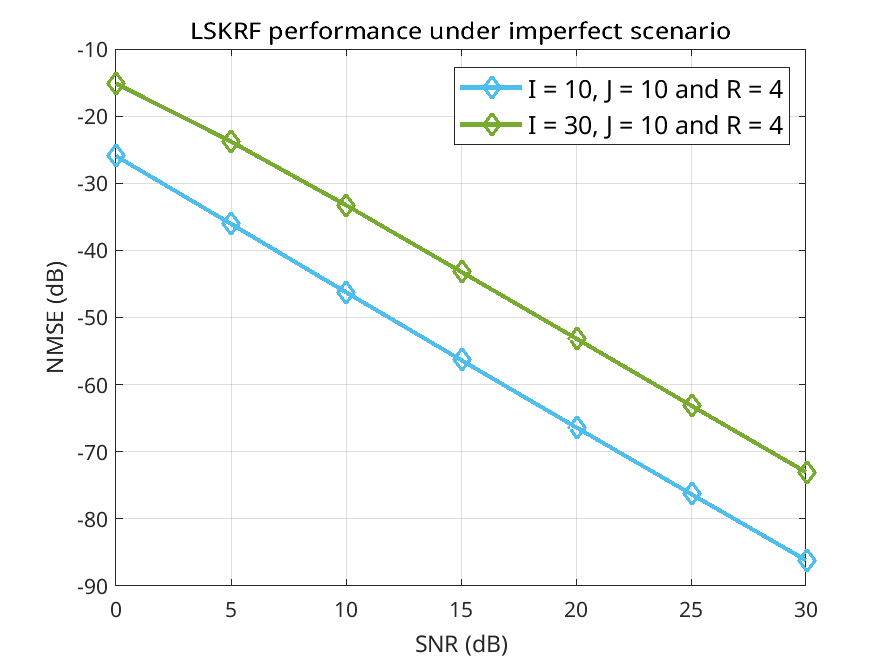
\includegraphics[width=0.75\linewidth]{figs/hw3.png} \par 
        \caption{Monter Carlo Experiment with 1000 runs for LSKRF algorithm.}
        \label{fig:hw3} 
    \end{figure}

    \newpage
    \subsection*{Produced Algorithm}

    \begin{verbatim}
        %% Least-Squares Khatri-Rao Factorization (LSKRF)

        % This function computes the LSKRF of a given matrix.   
        % Author: Kenneth B. dos A. Benicio <kenneth@gtel.ufc.br>
        % Created: February 2022

        function [Ahat,Bhat] = LSKRF(C,ia,ib)
            [~, jc] = size(C);
            
            Ahat = complex(zeros(ia,jc),0);
            Bhat = complex(zeros(ib,jc),0);
            
            for j = 1:jc
                Cp = C(:,j);
                Cp = reshape(Cp, [ib ia]);
                [U,S,V] = svd(Cp);
                Ahat(:,j) = sqrt(S(1,1)).*conj(V(:,1));
                Bhat(:,j) = sqrt(S(1,1)).*U(:,1);
            end
        end

        %% ----- Homework 3 ----- %%
        clc;
        clear;
        close all;

        A = randn(4,2) + 1j*randn(4,2);
        B = randn(6,2) + 1j*randn(6,2);
        X = tensor.mtx_prod_kr(A,B);
        [Ahat,Bhat] = tensor.LSKRF(X,4,6);
        Xhat = tensor.mtx_prod_kr(Ahat,Bhat);

        disp('Checking the NMSE (dB) between the original matrix X and its'... 
            'reconstruction with LSKRF:')
        nmsex = (norm(X- Xhat,'fro')^2)/(norm(X,'fro')^2);
        nmsex = 20*log10(nmsex)
        disp('Checking the NMSE (dB) between the original matrix A and its'...
            'estimation:')
        nmsea = (norm(A- Ahat,'fro')^2)/(norm(A,'fro')^2);
        nmsea = 20*log10(nmsea)
        disp('Checking the NMSE (dB) between the original matrix B and its'... 
            'estimation:')
        nmseb = (norm(B- Bhat,'fro')^2)/(norm(B,'fro')^2);
        nmseb = 20*log10(nmseb)

        I = 10;
        J = 10;
        R =  4;
        SNR = [0 5 10 15 20 25 30];
        nmse = zeros(length(SNR),1);
        for snr = 1:length(SNR)
            for mc = 1:1000
                var_noise = 1/(10^(SNR(snr)/10));
                noise = sqrt(var_noise/2)*(randn(I*J,R) + 1j*randn(I*J,R));
                
                A = randn(I,R) + 1j*randn(I,R);
                B = randn(J,R) + 1j*randn(J,R);
                X = tensor.mtx_prod_kr(A,B);
                X_noisy = X + noise;
                
                [Ahat,Bhat] = tensor.LSKRF(X_noisy,I,J);
                Xhat = tensor.mtx_prod_kr(Ahat,Bhat);
                aux = (norm(X- Xhat,'fro')^2)/(norm(X,'fro')^2);
                nmse(snr,1) = nmse(snr,1) + 20*log10(aux);
            end
        end
        nmse  = nmse/1000;

        figure
        txt = ['I = ' num2str(I), ', J = ' num2str(J), ' and R = ' num2str(R)];
        plot(SNR,nmse,'-d','color', [0.3010 0.7450 0.9330], "linewidth", 2,...
            "markersize", 8, "DisplayName", txt);
        hold on;

        I = 30;
        J = 10;
        R =  4;
        SNR = [0 5 10 15 20 25 30];
        nmse = zeros(length(SNR),1);
        for snr = 1:length(SNR)
            for mc = 1:1000
                var_noise = 1/(10^(SNR(snr)/10));
                noise = sqrt(var_noise/2)*(randn(I*J,R) + 1j*randn(I*J,R));
                
                A = randn(I,R) + 1j*randn(I,R);
                B = randn(J,R) + 1j*randn(J,R);
                X = tensor.mtx_prod_kr(A,B);
                X = X + noise;
                
                [Ahat,Bhat] = tensor.LSKRF(X,I,J);
                Xhat = tensor.mtx_prod_kr(Ahat,Bhat);
                aux = (norm(X- Xhat,'fro')^2)/(norm(X,'fro')^2);
                nmse(snr,1) = nmse(snr,1) + 20*log10(aux);
            end
        end
        nmse  = nmse/1000;

        txt = ['I = ' num2str(I), ', J = ' num2str(J), ' and R = ' num2str(R)];
        plot(SNR,nmse,'-d','color', [0.4660 0.6740 0.1880], "linewidth", 2,...
            "markersize", 8, "DisplayName", txt);
        hold off;
        title(['LSKRF performance under imperfect scenario'])
        xlabel('SNR (dB)')
        ylabel('NMSE (dB)')
        legend_copy = legend("location", "northwest");
        set(legend_copy,'Interpreter','tex','location','northeast',"fontsize", 12)
        grid on;
        saveas(gcf,'hw3.png')
    \end{verbatim}
    
\newpage
\section*{Homework 4 \\ Least Squares Kronecker Product Factorization (LSKronF)}

    \subsection*{Implementation LSKronF}

    The LSKronF algorithm aims to solve the following estimation problem 

    \begin{align}
        \left(\hat{\boldsymbol{A}}, \hat{\boldsymbol{B}}\right) = \underset{\boldsymbol{A}, \boldsymbol{B}}{\text{min}} \left|\left| \boldsymbol{X} - \boldsymbol{A} \otimes \boldsymbol{B} \right|\right|^2_{\text{F}},
    \end{align}

    and by implementing the algorithm it was possible to reach the following table of NMSE (dB) values using the validation files 

    \begin{table}[ht!]
        \centering
        \begin{tabular}{|l|l|l|l|}
        \hline
        NMSE($\boldsymbol{X}, \boldsymbol{\hat{X}}$) & NMSE($\boldsymbol{A}, \boldsymbol{\hat{A}}$) & NMSE($\boldsymbol{B}, \boldsymbol{\hat{B}}$) \\ \hline
        -619.2196 & +13.5472 & +9.5922 \\ \hline
        \end{tabular}
    \end{table}

    as we can see the estimation of the matrix $\boldsymbol{X}$ is perfect, but the estimated factor matrices are far from the original ones. This is simply explained by 
    the scale ambiguity intrinsic to the LSKronF. This could be eliminated if we assume previous knowledge of either the structure of the factor matrices or some of their elements.
    
    \subsection*{Monte Carlo Experiment}

    In Figure \ref{fig:hw4} the Monte Carlo Experiment is used to draw the curves for two different scenarios: $(I,J,P,Q) = (2,4,3,5)$ and $(I,J,P,Q) = (4,8,3,5)$. 
    As we can observe the best performance is the one where the algorithm have fewer elements to estimate. This is to be expected since the noise will have a lot less
    components that could potentially harm the performance of the LSKronF.

    \begin{figure}[ht!]
        \centering 
        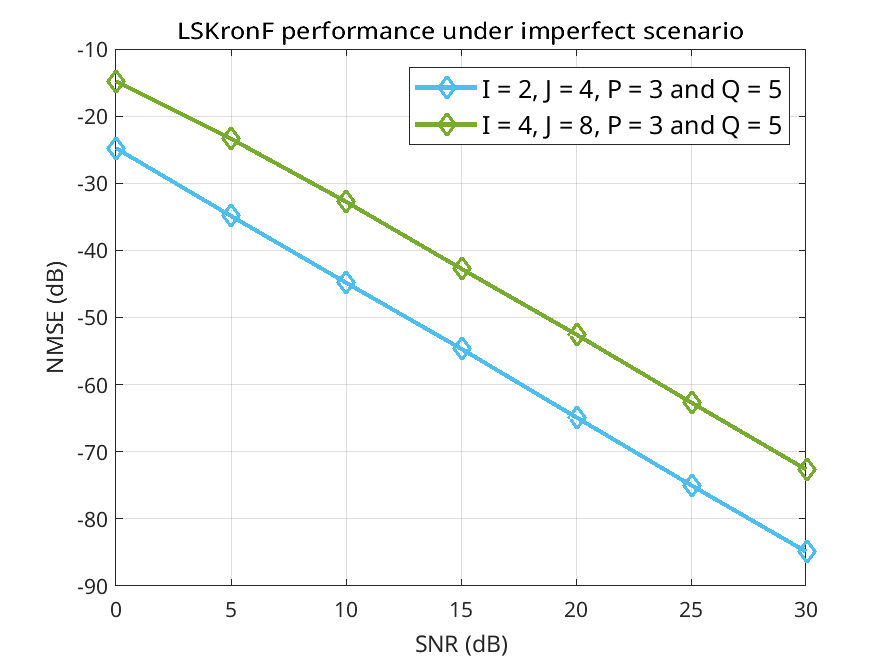
\includegraphics[width=0.75\linewidth]{figs/hw4.png} \par 
        \caption{Monter Carlo Experiment with 1000 runs for LSKronf algorithm.}
        \label{fig:hw4} 
    \end{figure}

    \newpage
    \subsection*{Produced Algorithm}

    \begin{verbatim}
        %% Least-Square Kronecker Product Factorization (LSKronF)

        % This function computes the LSKronF of a given matrix.   
        % Author: Kenneth B. dos A. Benicio <kenneth@gtel.ufc.br>
        % Created: February 2022

        function [Ahat,Bhat] = LSKronF(C,ia,ja,ib,jb)
            [ic,jc] = size(C);
            
            I = (ic/ia) + zeros(1,ia);
            J = (jc/ja) + zeros(1,ja);
            blocks_of_C = mat2cell(C,I,J);
            
            k = 1;
            Chat = complex(zeros(ib*jb,ia*ja),0);
            for j = 1:ja
                for i = 1:ia
                    vec_of_block = cell2mat(blocks_of_C(i,j));
                    vec_of_block = vec_of_block(:);
                    Chat(:,k) = vec_of_block;
                    k = k + 1;
                end
            end
            
            [U,S,V] = svd(Chat);
            ahat = sqrt(S(1,1)).*conj(V(:,1));
            bhat = sqrt(S(1,1)).*U(:,1);
            Ahat = reshape(ahat,[ia ja]);
            Bhat = reshape(bhat, [ib jb]);
        end

        %% ----- Homework 4 ----- %%
        clc;
        clear;
        close all;

        A = randn(4,2) + 1j*randn(4,2);
        B = randn(6,3) + 1j*randn(6,3);
        X = tensor.mtx_prod_kron(A,B);
        [Ahat,Bhat] = tensor.LSKronF(X,4,2,6,3);
        Xhat = tensor.mtx_prod_kron(Ahat,Bhat);

        disp('Checking the NMSE (dB) between the original matrix X and its'...
            'reconstruction with LSKronF:')
        nmsex = (norm(X- Xhat,'fro')^2)/(norm(X,'fro')^2);
        nmsex = 20*log10(nmsex)
        disp('Checking the NMSE (dB) between the original matrix A and its'...
            'estimation:')
        nmsea = (norm(A- Ahat,'fro')^2)/(norm(A,'fro')^2);
        nmsea = 20*log10(nmsea)
        disp('Checking the NMSE (dB) between the original matrix B and its'...
            'estimation:')
        nmseb = (norm(B- Bhat,'fro')^2)/(norm(B,'fro')^2);
        nmseb = 20*log10(nmseb)

        I = 2;
        J = 4;
        P = 3;
        Q = 5;
        SNR = [0 5 10 15 20 25 30];
        nmse = zeros(length(SNR),1);
        for snr = 1:length(SNR)
            for mc = 1:1000
                var_noise = 1/(10^(SNR(snr)/10));
                noise = sqrt(var_noise/2)*(randn(I*J,P*Q) + 1j*randn(I*J,P*Q));
                
                A = randn(I,P) + 1j*randn(I,P);
                B = randn(J,Q) + 1j*randn(J,Q);
                X = tensor.mtx_prod_kron(A,B);
                X_noisy = X + noise;
                
                [Ahat,Bhat] = tensor.LSKronF(X_noisy,I,P,J,Q);
                Xhat = tensor.mtx_prod_kron(Ahat,Bhat);
                aux = (norm(X- Xhat,'fro')^2)/(norm(X,'fro')^2);
                nmse(snr,1) = nmse(snr,1) + 20*log10(aux);
            end
        end
        nmse  = nmse/1000;

        figure
        txt = ['I = ' num2str(I), ', J = ' num2str(J), ', P = ' num2str(P),...
            ' and Q = ' num2str(Q)];
        plot(SNR,nmse,'-d','color', [0.3010 0.7450 0.9330], "linewidth", 2,...
            "markersize", 8, "DisplayName", txt);
        hold on;

        I = 4;
        J = 8;
        P = 3;
        Q = 5;
        SNR = [0 5 10 15 20 25 30];
        nmse = zeros(length(SNR),1);
        for snr = 1:length(SNR)
            for mc = 1:1000
                var_noise = 1/(10^(SNR(snr)/10));
                noise = sqrt(var_noise/2)*(randn(I*J,P*Q) + 1j*randn(I*J,P*Q));
                
                A = randn(I,P) + 1j*randn(I,P);
                B = randn(J,Q) + 1j*randn(J,Q);
                X = tensor.mtx_prod_kron(A,B);
                X = X + noise;
                
                [Ahat,Bhat] = tensor.LSKronF(X,I,P,J,Q);
                Xhat = tensor.mtx_prod_kron(Ahat,Bhat);
                aux = (norm(X- Xhat,'fro')^2)/(norm(X,'fro')^2);
                nmse(snr,1) = nmse(snr,1) + 20*log10(aux);
            end
        end
        nmse  = nmse/1000;

        txt = ['I = ' num2str(I), ', J = ' num2str(J), ', P = ' num2str(P),...
            ' and Q = ' num2str(Q)];
        plot(SNR,nmse,'-d','color', [0.4660 0.6740 0.1880], "linewidth", 2,...
            "markersize", 8, "DisplayName", txt);
        hold off;
        title(['LSKronF performance under imperfect scenario'])
        xlabel('SNR (dB)')
        ylabel('NMSE (dB)')
        legend_copy = legend("location", "northwest");
        set(legend_copy,'Interpreter','tex','location','northeast',"fontsize", 12)
        grid on;
        saveas(gcf,'hw4.png')
    \end{verbatim}
    
\newpage
\section*{Homework 5 \\ Kronecker Product Singular Value Decomposition (KPSVD)}

    \subsection*{Implementation and Validation of KPSVD}

    The KPSVD algorithm aims to solve the following estimation problem 

    \begin{align}
        \boldsymbol{X} = \sum^{r_{kp}}_{k = 1} \sigma_{k} \boldsymbol{U}_{k} \otimes \boldsymbol{V}_{k},
    \end{align}

    Since a validation file was not available I decided to create my own validation by generating a full-rank matrix with $R = 9$ and in sequence two approximations using my KPSVD implementation are provided: \
    One using the full-rank approximation and other using a r-rank approximation with $r \in \{1,3,5,7\}$. The NMSE (dB) between the original matriz $\boldsymbol{X}$ and its low-rank approximations are 
    shown in the following table

    \begin{table}[ht!]
        \centering
        \begin{tabular}{|l|l|l|l|l|}
        \hline
        r = 9 & r = $7$ & r = $5$ & r = $3$ & r = $1$ \\ \hline
        -604.8023 & -51.3722 & -26.7589 & -16.9054 & -6.3068 \\ \hline
        \end{tabular}
    \end{table}

    and as we can observe the low-rank approximations are not good enought mainly because we are working with a full-rank matrix. Thus, it would be expected to obtain a better
    performance for low-rank approximations of the matrix $\boldsymbol{X}$ if the matrix would to be rank defficient.

    \subsection*{Produced Algorithm}

    \begin{verbatim}
        %% Kronecker Product Single Value Decomposition (KPSVD)

        % This function computes the LSKRF of a given matrix.   
        % Author: Kenneth B. dos A. Benicio <kenneth@gtel.ufc.br>
        % Created: March 2022

        function [U,S,V,rkp] = KPSVD(X,ia,ja,ib,jb)
            [ix,jx] = size(X);
            
            I = (ix/ia) + zeros(1,ia);
            J = (jx/ja) + zeros(1,ja);
            blocks_of_X = mat2cell(X,I,J);
            
            k = 1;
            Xhat = complex(zeros(ib*jb,ia*ja),0);
            for j = 1:ja
                for i = 1:ia
                    vec_of_block = cell2mat(blocks_of_X(i,j));
                    vec_of_block = vec_of_block(:);
                    Xhat(:,k) = vec_of_block;
                    k = k + 1;
                end
            end
            [U,S,V] = svd(Xhat');
            rkp = sum(sum(S>0));
        end

        %% ----- Homework 5 ----- %%
        clc;        % This function computes the LSKRF of a given matrix.   
        % Author: Kenneth B. dos A. Benicio <kenneth@gtel.ufc.br>
        % Created: March 2022

        function [U,S,V,rkp] = KPSVD(X,ia,ja,ib,jb)
            [ix,jx] = size(X);
            
            I = (ix/ia) + zeros(1,ia);
            J = (jx/ja) + zeros(1,ja);
            blocks_of_X = mat2cell(X,I,J);
            
            k = 1;
            Xhat = complex(zeros(ib*jb,ia*ja),0);
            for j = 1:ja
                for i = 1:ia
                    vec_of_block = cell2mat(blocks_of_X(i,j));
                    vec_of_block = vec_of_block(:);
                    Xhat(:,k) = vec_of_block;
                    k = k + 1;
                end
            end
            [U,S,V] = svd(Xhat');
            rkp = sum(sum(S>0));
        end

        r1 = 3;
        c1 = 3;
        r2 = 3;
        c2 = 3;
        rank_of_A = 3;

        % Using the outer product between vectors to control the rank of a matrix.
        A = complex(zeros(r1*r2,c1*c2),0);
        for i = 1:rank_of_A
            aux1 = randn(r1*r2,1)+ 1i*randn(r1*r2,1); 
            aux2 = randn(1,c1*c2)+ 1i*randn(1,c1*c2); 
            A = A + aux1*aux2; 
        end
        [U,S,V,rkp] = tensor.KPSVD(A,r1,c1,r2,c2);

        % Reconstructing A with full rank.
        Ahat = complex(zeros(r1*r2,c1*c2),0);
        for r = 1:rkp
            aux1 = U(:,r);
            aux2 = conj(V(:,r));
            Uk{r} = reshape(aux1,[r1 c1]);
            Vk{r}  = reshape(aux2, [r2 c2]); 
            Ahat = Ahat + S(r,r)*tensor.mtx_prod_kron(Uk{r},Vk{r});
        end 
        disp('Checking the NMSE (dB) between the original matrix A and its'... 
            'reconstruction with KPSVD using full rank:')
        Ahat = conj(Ahat);
        nmse = (norm(A - Ahat,'fro')^2)/(norm(A,'fro')^2);
        nmse = 20*log10(nmse)

        % Reconstructing A with deficient rank.
        Ahat = complex(zeros(r1*r2,c1*c2),0);
        for r = 1:3
            aux1 = U(:,r);
            aux2 = conj(V(:,r));
            Uk{r} = reshape(aux1,[r1 c1]);
            Vk{r}  = reshape(aux2, [r2 c2]); 
            Ahat = Ahat + S(r,r)*tensor.mtx_prod_kron(Uk{r},Vk{r});
        end  
        disp('Checking the NMSE (dB) between the original matrix A and its'...
            'reconstruction with KPSVD using deficient rank:')
        Ahat = conj(Ahat);
        nmse = (norm(A - Ahat,'fro')^2)/(norm(A,'fro')^2);
        nmse = 20*log10(nmse)
    \end{verbatim}
    
\newpage
\section*{Homework 6 \\ Unfolding, folding, and n-mode product}

    \subsection*{Implementation and Validation of unfolding, folding and n-mode product}

    The unfolding, folding and n-mode product operations were implemented according the following prototype

    \begin{align}
        [\mathcal{X}]_{n} &= \text{unfold}(\mathcal{X}, [I_{1} \cdots I_{N} ], n) \in \mathbb{C}^{I_{n} \times I_{1} \cdots I_{n-1} I_{n+1} \cdots I_{N}}, \\
        \mathcal{X} &= \text{fold}([\mathcal{X}]_{n}, [I_{1} \cdots I_{N} ], n) \in \mathbb{C}^{I_{1} \times \cdots \times I_{N}}, \\
        \mathcal{Y} &= \mathcal{X} \times_{1} \boldsymbol{U}_{1} \times_{2} \cdots \times_{N} \boldsymbol{U}_{N},
    \end{align}

    and in sequence the provided files were used to validade the algorithms. As it will be possible to see by running the corresponde homework file ('homerwork6.m') it was 
    possible to validade all the algorithms. Nonentheless, all the three algorithms are generalized for $N$th order tensors and TensorLab was used to verify that.

    \subsection*{Produced Algorithm}

    \begin{verbatim}
        %% Unfolding

        % This function computes the unfolding of a given tensor in its matrix.   
        % Author: Kenneth B. dos A. Benicio <kenneth@gtel.ufc.br>
        % Created: April 2022

        function [A] = unfold(ten,mode)
            dim = size(ten);
            order = 1:numel(dim);
            order(mode) = [];
            order = [mode order];
            A = reshape(permute(ten,order), dim(mode), prod(dim)/dim(mode));
        end

        %% Folding

        % This function computes the folding of a given matrix into its tensor.   
        % Author: Kenneth B. dos A. Benicio <kenneth@gtel.ufc.br>
        % Created: April 2022

        % It's interesting to see how the dimmensions get swapped by the unfolding
        % so the understanding of the code is clear.
        function [ten] = fold(A,dim,mode)
            order = 1:numel(dim);
            order(mode) = [];
            order = [mode order];
            dim = dim(order);
            ten = reshape(A,dim);
            
            if mode == 1
                ten = permute(ten,order);
            else
                order = 1:numel(dim);
                for i = 2:mode
                    order([i-1 i]) = order([i i-1]);
                end
                ten = permute(ten,order);
            end
        end

        %% N-mode Product

        % This function computes n-mode product of a set of matrices and a tensor.   
        % Author: Kenneth B. dos A. Benicio <kenneth@gtel.ufc.br>
        % Created: April 2022

        function [ten] = n_mod_prod(ten,matrices,modes)
            dim = size(ten);
            number = numel(matrices);
            if nargin < 3
            modes = 1:number; 
            end
            
            for i = modes
                ten = cell2mat(matrices(i))*tensor.unfold(ten,i);
                [aux,~] = size(cell2mat(matrices(i)));
                dim(i) = aux;
                ten = tensor.fold(ten,[dim],i);
            end
        end

        %% ----- Homework 6 ----- %%
        clc;
        clear;
        close all;

        % Tensor for testing
        disp('Generic Tensor:');
        load('homework6_unfolding_folding.mat')
        dimension = size(tenX);

        % Kolda example for testing
        % load('homework6_kolda_example.mat')
        % tenX = xxx;
        % dimension = size(tenX);

        % Unfolding
        disp('X1./unfold(tenX,1):');
        tenX_1 = tensor.unfold(tenX,1);
        X1./tensor.unfold(tenX,1)
        disp('X2./unfold(tenX,2):');
        tenX_2 = tensor.unfold(tenX,2);
        X2./tensor.unfold(tenX,2)
        disp('X3./unfold(tenX,3):');
        tenX_3 = tensor.unfold(tenX,3);
        X3./tensor.unfold(tenX,3)

        % Folding
        disp('tenX./fold(unfold(tenX,1),1):');
        tenX./tensor.fold(tenX_1,dimension,1)
        disp('tenX./fold(unfold(tenX,2),2):');
        tenX./tensor.fold(tenX_2,dimension,2)
        disp('tenX./fold(unfold(tenX,3),3):');
        tenX./tensor.fold(tenX_3,dimension,3)

        % N-mode product
        load('homework6_n_mode.mat')
        tenY_test = tensor.n_mod_prod(tenX,{Z},[1]);
        disp('Checking the NMSE (dB) between the original tensor Y and the one'... 
            'after the N-mode product:')
        nmsey = (norm(tensor.unfold(tenY- tenY_test,1),'fro')^2)...
            /(norm(tensor.unfold(tenY,1),'fro')^2);
        nmsey = 20*log10(nmsey)
    \end{verbatim}
    
\newpage
\section*{Homework 7 \\ High Order Singular Value Decomposition (HOSVD)}

    \subsection*{Implementation HOSVD}

    \begin{table}[ht!]
        \centering
        \begin{tabular}{|l|l|l|l|l|}
        \hline
        NMSE($\mathcal{X}, \mathcal{\hat{X}}$) & NMSE($\mathcal{S}, \mathcal{\hat{S}}$) & NMSE($\boldsymbol{U}_{1}, \boldsymbol{\hat{U}}_{1}$) & NMSE($\boldsymbol{U}_{2}, \boldsymbol{\hat{U}}_{2}$) & NMSE($\boldsymbol{U}_{3}, \boldsymbol{\hat{U}}_{3}$) \\ \hline
        -611.2162 & +7.7656 & +2.6667 & +2.0000 & +1.6063 \\ \hline
        \end{tabular}
    \end{table}

    \subsection*{Validation of HOSVD}
    
    The multilinear rank advantage is maximized when it comes to process sparce tensors since the dimmensions can be greatly reduced without losing of too much relevant information by analysing the profile of its multiples unfoldings.

    \begin{align}
        \mathcal{X} &\in \mathbb{C}^{8 \times 4 \times 10} \to \hat{\mathcal{X}} \in \mathbb{C}^{R_{1} \times R_{2} \times R_{3}}, \\ 
        \mathcal{X} &\in \mathbb{C}^{5 \times 5 \times 5} \to \hat{\mathcal{Y}} \in \mathbb{C}^{P_{1} \times P_{2} \times P_{3}},
    \end{align}

    \newpage
    \subsection*{Produced Algorithm}

    \begin{verbatim}
        %% Full High Order Single Value Decomposition (HOSVD)

        % This function computes the Truncated HOSVD of a given tensor.   
        % Author: Kenneth B. dos A. Benicio <kenneth@gtel.ufc.br>
        % Created: April 2022

        function [S,U] = HOSVD_full(ten)
            number = numel(size(ten));
            for i = 1:number
            [aux,~,~] = svd(tensor.unfold(ten,i)); 
            %[aux,~,~] = svd(tens2mat(ten,i)); 
            U{i} = aux;
            end
            % Core tensor uses the hermitian operator.
            Ut = cellfun(@(x) x', U,'UniformOutput',false); 
            S = tensor.n_mod_prod(ten,Ut);
            % The normal factors should be transposed.
            U = cellfun(@(x) x, U,'UniformOutput',false);  
        end

        %% Truncated High Order Single Value Decomposition (HOSVD)

        % This function computes the Truncated HOSVD of a given tensor.   
        % Author: Kenneth B. dos A. Benicio <kenneth@gtel.ufc.br>
        % Created: April 2022

        function [S,U] = HOSVD_truncated(ten,ranks)
            if nargin < 2
                number = numel(size(ten));
                for i = 1:number
                [aux,eig,~] = svd(tensor.unfold(ten,i)); 
                [aa,~] = size(eig(eig > eps));
                aux = aux(:,1:aa);
                U{i} = aux;
                end
                % Core tensor uses the hermitian operator.
                Ut = cellfun(@(x) x', U,'UniformOutput',false); 
                S = tensor.n_mod_prod(ten,Ut);
                % The normal factors should be transposed.
                U = cellfun(@(x) x, U,'UniformOutput',false);
            else
                number = numel(size(ten));
                for i = 1:number
                [aux,~,~] = svd(tensor.unfold(ten,i)); 
                aux = aux(:,1:ranks(i));
                U{i} = aux;
                end
                % Core tensor uses the hermitian operator.
                Ut = cellfun(@(x) x',U,'UniformOutput',false); 
                S = tensor.n_mod_prod(ten,Ut);
                % The normal factors should be transposed.
                U = cellfun(@(x) x,U,'UniformOutput',false);
            end    
        end

        %% ----- Homework 7 ----- %%
        clc;
        clear;
        close all;

        % Full HOSVD
        load('homework7_HOSVD.mat');
        [tenS_hat,U_hat] = tensor.HOSVD_full(tenX);
        tenX_hat = tensor.n_mod_prod(tenS_hat,U_hat);

        % Checking the orthogonality
        disp('Checking the orthogonality propertie between the subtensors'...
            'formed from the core tensor:')
        reshape(tenS_hat(:,:,1),[],1)'*reshape(tenS_hat(:,:,4),[],1)

        disp('Checking the NMSE (dB) between the original tensor X and its'... '
            reconstruction:')
        nmsex = (norm(tensor.unfold(tenX - tenX_hat,1),'fro')^2)...
            /(norm(tensor.unfold(tenX,1),'fro')^2);
        nmsex = 20*log10(nmsex)
        disp('Checking the NMSE (dB) between the original core tensor S and its'... 
            'reconstruction:')
        nmses = (norm(tensor.unfold(tenS - tenS_hat,1),'fro')^2)...
            /(norm(tensor.unfold(tenS,1),'fro')^2);
        nmses = 20*log10(nmses)

        disp('Checking the NMSE (dB) between the original matrices and its'... 
            'estimations:')
        nmseU1 = (norm(U1 - U_hat{1},'fro')^2)/(norm(U1,'fro')^2)
        nmseU2 = (norm(U2 - U_hat{2},'fro')^2)/(norm(U2,'fro')^2)
        nmseU3 = (norm(U3 - U_hat{3},'fro')^2)/(norm(U3,'fro')^2)

        % Truncated HOSVD and Denoising
        X = randn(8,4,10) + 1i*randn(8,4,10);
        Y = randn(5,5,5) + 1i*randn(5,5,5);

        [S1,U1] = tensor.HOSVD_truncated(X);
        multilinear_rank1 = size(S1);
        [S2,U2] = tensor.HOSVD_truncated(Y);
        multilinear_rank2 = size(S2);

        Xhat = tensor.n_mod_prod(S1,U1);
        Yhat = tensor.n_mod_prod(S2,U2);

        disp('Checking the NMSE (dB) between the original noisy tensor X and'... 
            'its reconstruction:')
        nmsex = (norm(tensor.unfold(X- Xhat,1),'fro')^2)...
            /(norm(tensor.unfold(X,1),'fro')^2);
        nmsex = 20*log10(nmsex)
        disp('Checking the NMSE (dB) between the original noisy tensor Y'...
            'and its reconstruction:')
        nmsey = (norm(tensor.unfold(Y- Yhat,1),'fro')^2)...
            /(norm(tensor.unfold(Y,1),'fro')^2);
        nmsey = 20*log10(nmsey)

        disp('The multilinear rank for the tensor X is:')
        size(S1)
        disp('The multilinear rank for the tensor Y is:')
        size(S2)
    \end{verbatim}
    
\newpage
\section*{Homework 8 \\ High Order Order Orthogonal Iteration (HOOI)}

    \subsection*{Implementation HOOI}

    \begin{table}[ht!]
        \centering
        \begin{tabular}{|l|l|l|l|l|}
        \hline
        NMSE($\mathcal{X}, \mathcal{\hat{X}}$) & NMSE($\mathcal{S}, \mathcal{\hat{S}}$) & NMSE($\boldsymbol{U}_{1}, \boldsymbol{\hat{U}}_{1}$) & NMSE($\boldsymbol{U}_{2}, \boldsymbol{\hat{U}}_{2}$) & NMSE($\boldsymbol{U}_{3}, \boldsymbol{\hat{U}}_{3}$) \\ \hline
        -607.9515 & +7.2483 & +2.6667 & +3.9622 & +1.16160 \\ \hline
        \end{tabular}
    \end{table}

    \subsection*{Validation of HOOI}

    The multilinear rank advantage is maximized when it comes to process sparce tensors since the dimmensions can be greatly reduced without losing of too much relevant information by analysing the profile of its multiples unfoldings.

    \begin{align}
        \mathcal{X} &\in \mathbb{C}^{8 \times 4 \times 10} \to \hat{\mathcal{X}} \in \mathbb{C}^{R_{1} \times R_{2} \times R_{3}}, \\ 
        \mathcal{X} &\in \mathbb{C}^{5 \times 5 \times 5} \to \hat{\mathcal{Y}} \in \mathbb{C}^{P_{1} \times P_{2} \times P_{3}},
    \end{align}

    \newpage
    \subsection*{Produced Algorithm}

    \begin{verbatim}
        %% High Order Orthogonal Iteration (HOOI)

        % This function computes the HOOI of a given tensor.   
        % Author: Kenneth B. dos A. Benicio <kenneth@gtel.ufc.br>
        % Created: May 2022

        function [S,U,k] = HOOI_full(ten)
            max_iter = 10;
            [~, U] = tensor.HOSVD_full(ten);
            number = numel(size(ten));
            for k = 1:max_iter
                for i = 1:number
                    modes = 1:number;
                    modes(i) = []; % It will skip this mode in the n_mod_prod.
                    Un = tensor.n_mod_prod(ten,U,modes);
                    [aux,~,~] = svd(tensor.unfold(Un,i));
                    U{i} = aux;
                end
            end
            % The conjugate transpose
            Ut = cellfun(@(x) x', U ,'UniformOutput',false);
            S = tensor.n_mod_prod(ten,Ut); 
        end

        %% Truncated High Order Orthogonal Iteration (HOOI)

        % This function computes the Truncated HOOI of a given tensor.   
        % Author: Kenneth B. dos A. Benicio <kenneth@gtel.ufc.br>
        % Created: May 2022

        function [S,U] = HOOI_truncated(ten,ranks)
            if nargin < 2
                max_iter = 10;
                [~, U] = tensor.HOSVD_full(ten);
                number = numel(size(ten));
                for k = 1:max_iter
                    for i = 1:number
                        modes = 1:number;
                        modes(i) = []; % It will skip this mode in the n_mod_prod.
                        Un = tensor.n_mod_prod(ten,U,modes);
                        [aux,eig,~] = svd(tensor.unfold(Un,i));
                        [aa,~] = size(eig(eig > eps));
                        U{i} = aux(:,1:aa);
                    end
                end
                % The conjugate transpose
                Ut = cellfun(@(x) x', U ,'UniformOutput',false);
                S = tensor.n_mod_prod(ten,Ut); 
            else
                max_iter = 10;
                [~, U] = tensor.HOSVD_full(ten);
                number = numel(size(ten));
                for k = 1:max_iter
                    for i = 1:number
                        modes = 1:number;
                        modes(i) = []; % It will skip this mode in the n_mod_prod.
                        Un = tensor.n_mod_prod(ten,U,modes);
                        [aux,~,~] = svd(tensor.unfold(Un,i));
                        U{i} = aux(:,1:ranks(i));
                    end
                end
                % The conjugate transpose
                Ut = cellfun(@(x) x', U ,'UniformOutput',false);
                S = tensor.n_mod_prod(ten,Ut); 
            end    
        end

        %% ----- Homework 8 ----- %%
        clc;
        clear;
        close all;

        % Full HOSVD
        load('homework8_HOOI.mat');
        [tenS_hat,U_hat] = tensor.HOOI_full(tenX);
        tenX_hat = tensor.n_mod_prod(tenS_hat,U_hat);

        % Checking the orthogonality
        disp('Checking the orthogonality propertie between the subtensors'...
            'formed from the core tensor:')
        reshape(tenS_hat(:,:,1),[],1)'*reshape(tenS_hat(:,:,4),[],1)

        disp('Checking the NMSE (dB) between the original tensor X and'...
            'its reconstruction:')
        nmsex = (norm(tensor.unfold(tenX - tenX_hat,1),'fro')^2)...
            /(norm(tensor.unfold(tenX,1),'fro')^2);
        nmsex = 20*log10(nmsex)
        disp('Checking the NMSE (dB) between the original core tensor S'...
            'and its reconstruction:')
        nmses = (norm(tensor.unfold(tenS - tenS_hat,1),'fro')^2)...
            /(norm(tensor.unfold(tenS,1),'fro')^2);
        nmses = 20*log10(nmses)

        disp('Checking the NMSE (dB) between the original matrices and'...
            'its estimations:')
        nmseU1 = (norm(U1 - U_hat{1},'fro')^2)/(norm(U1,'fro')^2)
        nmseU2 = (norm(U2 - U_hat{2},'fro')^2)/(norm(U2,'fro')^2)
        nmseU3 = (norm(U3 - U_hat{3},'fro')^2)/(norm(U3,'fro')^2)

        % Truncated HOSVD and Denoising
        X = randn(8,4,10) + 1i*randn(8,4,10);
        Y = randn(5,5,5) + 1i*randn(5,5,5);

        [S1,U1] = tensor.HOOI_truncated(X);
        multilinear_rank1 = size(S1);
        [S2,U2] = tensor.HOOI_truncated(Y);
        multilinear_rank2 = size(S2);

        Xhat = tensor.n_mod_prod(S1,U1);
        Yhat = tensor.n_mod_prod(S2,U2);

        disp('Checking the NMSE (dB) between the original noisy tensor X and'...
            its reconstruction:')
        nmsex = (norm(tensor.unfold(X- Xhat,1),'fro')^2)...
            /(norm(tensor.unfold(X,1),'fro')^2);
        nmsex = 20*log10(nmsex)
        disp('Checking the NMSE (dB) between the original noisy tensor Y'...
            'and its reconstruction:')
        nmsey = (norm(tensor.unfold(Y- Yhat,1),'fro')^2)...
            /(norm(tensor.unfold(Y,1),'fro')^2);
        nmsey = 20*log10(nmsey)

        disp('The multilinear rank for the tensor X is:')
        size(S1)
        disp('The multilinear rank for the tensor Y is:')
        size(S2)
    \end{verbatim}
    
\newpage
\section*{Homework 9 \\ Multidimensional Least-Squares Khatri-Rao Factorization
(MLS-KRF)}

    \subsection*{Implementation MLS-KRF}
        
    The MLS-KRF algorithm aims to solve the following estimation problem 
    
    \begin{align}
        \left(\hat{\boldsymbol{A}}^{(1)}, \cdots, \hat{\boldsymbol{A}}^{(N)}\right) = \underset{\boldsymbol{A}^{(1)}, \cdots, \boldsymbol{A}^{(N)}}{\text{min}} \left|\left| \boldsymbol{X} - \boldsymbol{A}^{(1)} \diamond \cdots \diamond \boldsymbol{A}^{(N)} \right|\right|^2_{\text{F}},
    \end{align}

    and by implementing the algorithm it was possible to reach the following table of NMSE (dB) values using the validation files 

    \begin{table}[ht!]
        \centering
        \begin{tabular}{|l|l|l|l|}
        \hline
        NMSE($\boldsymbol{X}, \boldsymbol{\hat{X}}$) & NMSE($\boldsymbol{A}_{1}, \boldsymbol{\hat{A}}_{1}$) & NMSE($\boldsymbol{A}_{2}, \boldsymbol{\hat{A}}_{2}$) & NMSE($\boldsymbol{A}_{3}, \boldsymbol{\hat{A}}_{3}$) \\ \hline
        -606.2255 & +3.1432 & +5.0165 & +4.7297 \\ \hline
        \end{tabular}
    \end{table}

    as we can see the estimation of the matrix $\boldsymbol{X}$ is perfect, but the estimated factor matrices are far from the original ones. This is simply explained by 
    the scale ambiguity intrinsic to the MLS-KRF. This could be eliminated if we assume previous knowledge of either the structure of the factor matrices or some of their elements.
    It is also important to say that the produced algorithm was generalized for a random number of factors.

    \subsection*{Monte Carlo Experiment}

    In Figure \ref{fig:hw9} the Monte Carlo Experiment is used to draw the curve for the scenario $(I_{1},I_{2},I_{3},R) = (2,3,4,4)$.
    As we can observe in this simple channel model the MLSKRF reaches a decent performance. Of course that this is only possible because the original matrix $\boldsymbol{X}$ has
    a strong Khatri-Rao structure, but if by some reason the channel or the noise could disrupt this structure (as in the low-snr scenario that we can analyze in the same figure) 
    then the performance could be an impediment for certain applications. 

    \begin{figure}[ht!]
        \centering 
        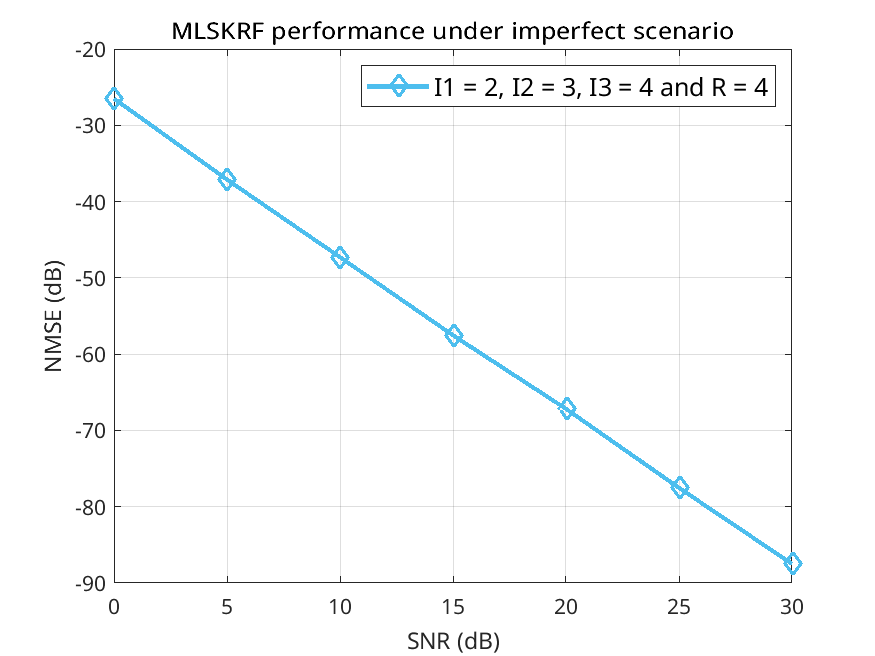
\includegraphics[width=0.65\linewidth]{figs/hw9.png} \par 
        \caption{Monter Carlo Experiment with 1000 runs for MLS-KRF algorithm.}
        \label{fig:hw9} 
    \end{figure}

    \newpage
    \subsection*{Produced Algorithm}

    \begin{verbatim}
        %% Multidimensional Least-Squares Khatri-Rao Factorization (MLS-KRF)

        % This function computes the MLS-KRF of a given matrix.   
        % Author: Kenneth B. dos A. Benicio <kenneth@gtel.ufc.br>
        % Created: March 2022

        % The dimensions should be inserted in the order that the products are
        % performed.
        function [A] = MLSKRF(X,N,dim)
            [~,R] = size(X); 
            for r = 1:R
                xr = X(:,r);
                tenXr = reshape(xr,flip(dim));
                
                % Aplicar SVDs consecutivas em estrategia recursiva? Como lidar com
                % o nd  array nesse caso?
                [Sr,Ur] = tensor.HOSVD_full(tenXr);
                for n = 1:N
                    Ar{r,n} = (Sr(1)^(1/N))*Ur{N - n + 1}(:,1);
                end
            end
            
            for n = 1:N
            aux = cell2mat(Ar(:,n)); 
            A{n} = reshape(aux,[dim(n) R]);
            end
        end

        %% ----- Homework 9 ----- %%
        clc;
        clear;
        close all;

        load('homework9_MLSKRF.mat')

        N = 3;
        dim = [5 4 8];
        [Matrices] = tensor.MLSKRF(X,N,dim); 
        Xhat = tensor.mtx_prod_kr(Matrices{1},Matrices{2});
        Xhat = tensor.mtx_prod_kr(Xhat,Matrices{3});

        disp(['Checking the NMSE (dB) between the original matrix X and its'...
            'reconstruction with MLSKRF:'])
        nmsex = (norm(X - Xhat,'fro')^2)/(norm(X,'fro')^2);
        nmsex = 20*log10(nmsex)
        disp(['Checking the NMSE (dB) between the original matrix A and its'...
            'estimation:'])
        nmsea = (norm(A - Matrices{1},'fro')^2)/(norm(A,'fro')^2);
        nmsea = 20*log10(nmsea)
        disp(['Checking the NMSE (dB) between the original matrix B and its'...
            'estimation:'])
        nmseb = (norm(B - Matrices{2},'fro')^2)/(norm(B,'fro')^2);
        nmseb = 20*log10(nmseb)
        disp(['Checking the NMSE (dB) between the original matrix C and its'...
            'estimation:'])
        nmsec = (norm(C - Matrices{3},'fro')^2)/(norm(C,'fro')^2);
        nmsec = 20*log10(nmsec)

        %% Monte Carlo Experiment
        N = 3;
        R  = 4;
        I = 2;
        J = 3;
        K = 4;
        dim = [I J K];
        SNR = [0 5 10 15 20 25 30];
        nmse = zeros(length(SNR),1);
        for snr = 1:length(SNR)
            for mc = 1:1000
                var_noise = 1/(10^(SNR(snr)/10));
                noise = sqrt(var_noise/2)*(randn(I*J*K,R) + 1j*randn(I*J*K,R));
                
                A = randn(I,R) + 1j*randn(I,R);
                B = randn(J,R) + 1j*randn(J,R);
                C = randn(K,R) + 1j*randn(K,R);
                X = tensor.mtx_prod_kr(A,B);
                X = tensor.mtx_prod_kr(X,C);
                X_noisy = X + noise;
                
                [Matrices] = tensor.MLSKRF(X_noisy,N,dim);
                Xhat = tensor.mtx_prod_kr(Matrices{1},Matrices{2});
                Xhat = tensor.mtx_prod_kr(Xhat,Matrices{3});
                aux = (norm(X- Xhat,'fro')^2)/(norm(X,'fro')^2);
                nmse(snr,1) = nmse(snr,1) + 20*log10(aux);
            end
        end
        nmse  = nmse/1000;

        figure
        txt = ['I1 = ' num2str(I), ', I2 = ' num2str(J), ', I3 = ' num2str(K),...
            ' and R = ' num2str(R)];
        plot(SNR,nmse,'-d','color', [0.3010 0.7450 0.9330], "linewidth", 2,...
            "markersize", 8, "DisplayName", txt);
        title(['MLSKRF performance under imperfect scenario'])
        xlabel('SNR (dB)')
        ylabel('NMSE (dB)')
        legend_copy = legend("location", "northwest");
        set(legend_copy,'Interpreter','tex','location','northeast',"fontsize", 12)
        grid on;
        saveas(gcf,'hw9.png')
    \end{verbatim}
    
\newpage
\section*{Homework 10 \\ Multidimensional Least-Squares Kronecker Factorization
(MLS-KronF)}

    \subsection*{Implementation MLS-KronF}

    The MLS-KronF algorithm aims to solve the following estimation problem 

    \begin{align}
        \left(\hat{\boldsymbol{A}}^{(1)}, \cdots, \hat{\boldsymbol{A}}^{(N)}\right) = \underset{\boldsymbol{A}^{(1)}, \cdots, \boldsymbol{A}^{(N)}}{\text{min}} \left|\left| \boldsymbol{X} - \boldsymbol{A}^{(1)} \otimes \cdots \otimes \boldsymbol{A}^{(N)} \right|\right|^2_{\text{F}},
    \end{align}

    and by implementing the algorithm it was possible to reach the following table of NMSE (dB) values using the validation files 
    for the HOSVD and HOOI initialization, respectively.

    \begin{table}[ht!]
        \centering
        \begin{tabular}{|l|l|l|l|}
        \hline
        NNMSE($\boldsymbol{X}, \boldsymbol{\hat{X}}$) & NMSE($\boldsymbol{A}_{1}, \boldsymbol{\hat{A}}_{1}$) & NMSE($\boldsymbol{A}_{2}, \boldsymbol{\hat{A}}_{2}$) & NMSE($\boldsymbol{A}_{3}, \boldsymbol{\hat{A}}_{3}$) \\ \hline
        -605.1941 & +11.9214 & +11.5548 & +6.0950 \\ \hline
        \end{tabular}
    \end{table}

    \begin{table}[ht!]
        \centering
        \begin{tabular}{|l|l|l|l|}
        \hline
        NNMSE($\boldsymbol{X}, \boldsymbol{\hat{X}}$) & NMSE($\boldsymbol{A}_{1}, \boldsymbol{\hat{A}}_{1}$) & NMSE($\boldsymbol{A}_{2}, \boldsymbol{\hat{A}}_{2}$) & NMSE($\boldsymbol{A}_{3}, \boldsymbol{\hat{A}}_{3}$) \\ \hline
        -608.4705 & +5.4597 & +15.0478 & +5.8977 \\ \hline
        \end{tabular}
    \end{table}

    as we can see the estimation of the matrix $\boldsymbol{X}$ is perfect, but the estimated factor matrices are far from the original ones for both cases. This is simply explained by 
    the scale ambiguity intrinsic to the MLS-KronF. This could be eliminated if we assume previous knowledge of either the structure of the factor matrices or some of their elements.
    It is also important to say that the produced algorithm was generalized for a random number of factors.

    \subsection*{Monte Carlo Experiment}

    In Figures \ref{fig:hw10a1}, \ref{fig:hw10a2}, \ref{fig:hw10a3} and \ref{fig:hw10a4} the Monte Carlo Experiment is used to draw the curves for the scenarios 
    $(I_{1},I_{2},I_{3}) = (J_{1},J_{2},J_{3}) = \{(2,2,2), (5,5,5), (2,3,4)\}$ and $(I_{1},I_{2},I_{3}) = (2,3,4), (J_{1},J_{2},J_{3}) = (5,6,7)$ for both the HOSVD and HOOI initializations. 
    As we can observe in  this simple channel model the MLSKronF reaches a decent performance. Of course that this is only possible because the original matrix $\boldsymbol{X}$ has a strong 
    Kronecker structure, but if by some reason the channel or the noise could disrupt this structure (as it can be seen in the low-snr scenarios) then the performance could be an impediment for certain applications.
    Its also interesting to note that all for all the scenarios it was not possible to verify any significant difference between the two methods of initialization of the MLSKronF.

    \begin{figure*}
        \centering
        \begin{subfigure}[b]{0.475\textwidth}
            \centering
            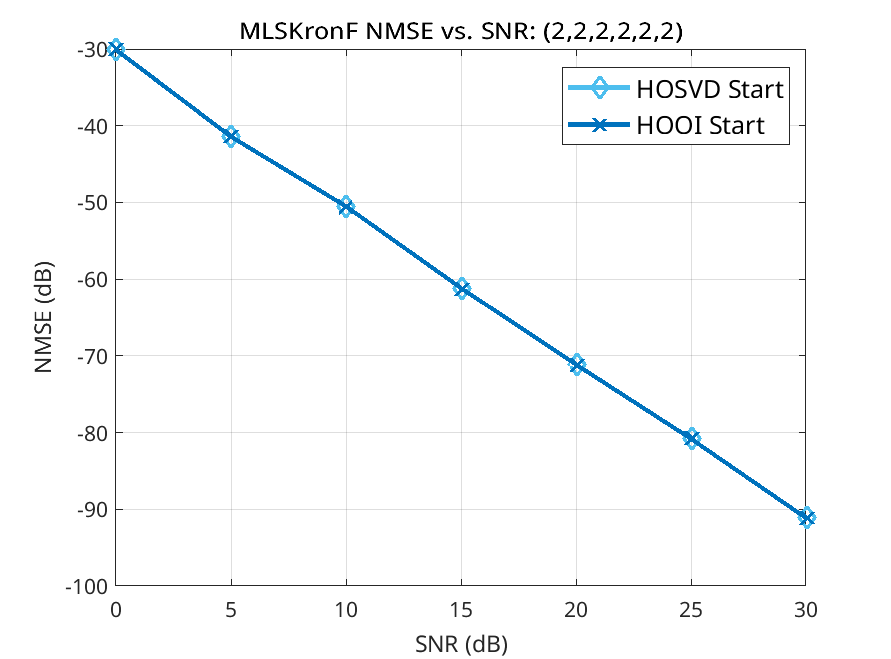
\includegraphics[width=\textwidth]{figs/hw10a1.png} 
            \caption[]%
            {{\small Scenario 1}}    
            \label{fig:hw10a1} 
        \end{subfigure}
        \hfill
        \begin{subfigure}[b]{0.475\textwidth}  
            \centering 
            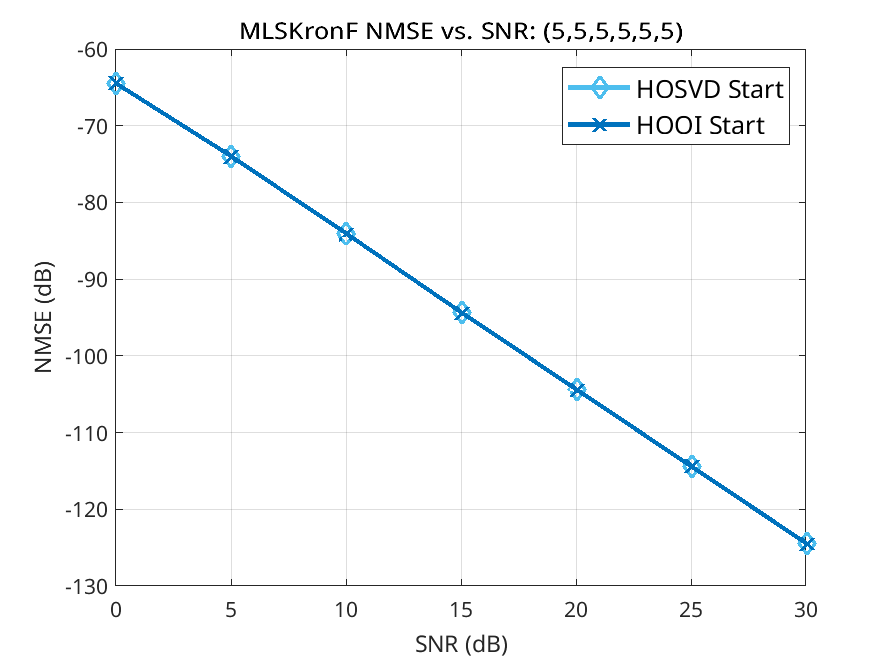
\includegraphics[width=\textwidth]{figs/hw10a2.png} 
            \caption[]%
            {{\small Scenario 2}}    
            \label{fig:hw10a2} 
        \end{subfigure}
        \vskip\baselineskip
        \begin{subfigure}[b]{0.475\textwidth}   
            \centering 
            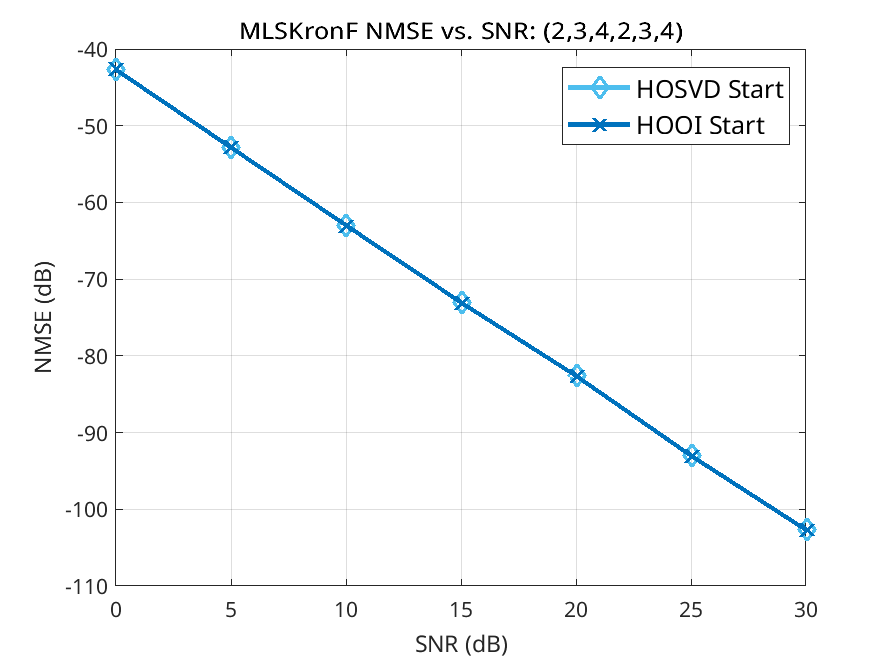
\includegraphics[width=\textwidth]{figs/hw10a3.png} 
            \caption[]%
            {{\small Scenario 3}}    
            \label{fig:hw10a3} 
        \end{subfigure}
        \hfill
        \begin{subfigure}[b]{0.475\textwidth}   
            \centering 
            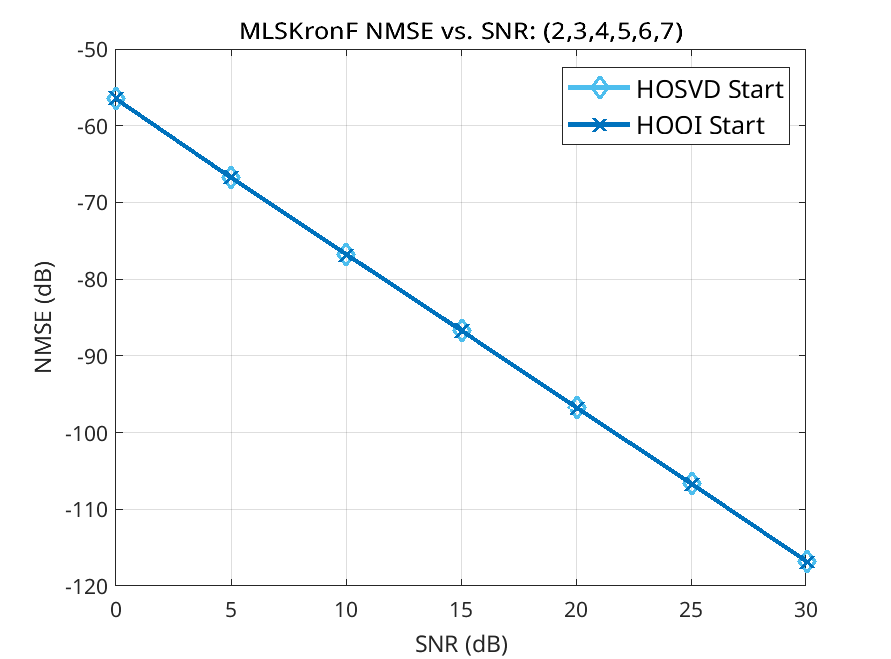
\includegraphics[width=\textwidth]{figs/hw10a4.png} 
            \caption[]%
            {{\small Scenario 4}}    
            \label{fig:hw10a4} 
        \end{subfigure}
        \caption[Monter Carlo Experiment with 1000 runs for MLS-KronF algorithm.]
        {\small Monter Carlo Experiment with 1000 runs for MLS-KronF algorithm.} 
        \label{fig:mean and std of nets}
    \end{figure*}

    

    \newpage
    \subsection*{Produced Algorithm}

    \begin{verbatim}
        %% Multidimensional Least-Squares Kronecker Factorization (MLS-KronF)

        % This function computes the MLS-KronF of a given matrix.   
        % Author: Kenneth B. dos A. Benicio <kenneth@gtel.ufc.br>
        % Created: March 2022
        
        % It is interesting to note that this process could easily be applied to a
        % random number of matrices in a iterative form considering groups of 3 objects.
        % init controls the initialization: 1 for HOSVD and 2 for HOOI.
        function [Ahat] = MLSKronF(X,rows,columns,init)
            % 3rd structure
            %[ix,jx] = size(X);
            
            % 2nd structure
            I = rows(2)*rows(3) + zeros(1,rows(1));
            J = columns(2)*columns(3) + zeros(1,columns(1));
            blocks_of_X = mat2cell(X,I,J);
            
            % 1st structure
            Z = 1;
            for j = 1:columns(1)
                for i = 1:rows(1)
                aux = cell2mat(blocks_of_X(i,j));
                I = rows(3) + zeros(1,rows(2));
                J = columns(3) + zeros(1,columns(2));
                blocks_of_aux = mat2cell(aux,I,J);
                for jj = 1:columns(2)
                        for ii = 1:rows(2)
                            vec_of_block = cell2mat(blocks_of_aux(ii,jj));
                            vec_of_block = vec_of_block(:);
                            mtx_1st(:,ii,jj) = vec_of_block;
                        end
                end
                    Xhat(:,Z) = reshape(mtx_1st,[],1);
                    Z = Z + 1;
                end 
            end
            
            tenXhat = reshape(Xhat,[rows(3)*columns(3), rows(2)*columns(2), rows(1)*columns(1)]);
            if init == '1'
                [S,U] = tensor.HOSVD_full(tenXhat);
            elseif init == '2'
                [S,U] = tensor.HOOI_full(tenXhat);
            end
            rows = flip(rows);
            columns = flip(columns);
            for u = 1:length(U)
                index = length(U) - u + 1;
                aux = (S(1)^(1/length(U)))*U{u}(:,1);
                Ahat{index} = reshape(aux,[rows(u) columns(u)]);
            end
        end

        %% ----- Homework 10 ----- %%
        clc;
        clear;
        close all;

        load('homework_10_MLSKronF.mat')

        rows = [4 4 6];
        columns = [3 2 5];

        %% Initialization by HOSVD
        [Matrices] = tensor.MLSKronF(X,rows,columns,'1');
        aux1 = tensor.mtx_prod_kron(Matrices{1},Matrices{2});
        Xhat = tensor.mtx_prod_kron(aux1,Matrices{3});
        disp(['Checking the NMSE (dB) between the original matrix X and its'...
            'reconstruction with MLSKronF:'])
        nmse1 = (norm(X - Xhat,'fro')^2)/(norm(X,'fro')^2);
        nmse1 = 20*log10(nmse1)
        disp(['Checking the NMSE (dB) between the original matrix A and its'...
            'estimation:'])
        nmsea = (norm(A - Matrices{1},'fro')^2)/(norm(A,'fro')^2);
        nmsea = 20*log10(nmsea)
        disp(['Checking the NMSE (dB) between the original matrix B and its'...
            'estimation:'])
        nmseb = (norm(B - Matrices{2},'fro')^2)/(norm(B,'fro')^2);
        nmseb = 20*log10(nmseb)
        disp(['Checking the NMSE (dB) between the original matrix C and its'...
            'estimation:'])
        nmsec = (norm(C - Matrices{3},'fro')^2)/(norm(C,'fro')^2);
        nmsec = 20*log10(nmsec)

        %% Initialization by HOOI
        [Matrices] = tensor.MLSKronF(X,rows,columns,'2');
        aux1 = tensor.mtx_prod_kron(Matrices{1},Matrices{2});
        Xhat = tensor.mtx_prod_kron(aux1,Matrices{3});
        disp(['Checking the NMSE (dB) between the original matrix X and its'...
            'reconstruction with MLSKronF:'])
        nmse1 = (norm(X - Xhat,'fro')^2)/(norm(X,'fro')^2);
        nmse1 = 20*log10(nmse1)
        disp(['Checking the NMSE (dB) between the original matrix A and its'...
            'estimation:'])
        nmsea = (norm(A - Matrices{1},'fro')^2)/(norm(A,'fro')^2);
        nmsea = 20*log10(nmsea)
        disp(['Checking the NMSE (dB) between the original matrix B and its'...
            'estimation:'])
        nmseb = (norm(B - Matrices{2},'fro')^2)/(norm(B,'fro')^2);
        nmseb = 20*log10(nmseb)
        disp(['Checking the NMSE (dB) between the original matrix C and its'...
            'estimation:'])
        nmsec = (norm(C - Matrices{3},'fro')^2)/(norm(C,'fro')^2);
        nmsec = 20*log10(nmsec)

        %% Monte Carlo Experiment
        ia = 2;
        ib = 2;
        ic = 2;
        ja = 2;
        jb = 2;
        jc = 2;
        rows = [ia ib ic];
        columns = [ja jb jc];
        SNR = [0 5 10 15 20 25 30];
        nmse1 = zeros(length(SNR),1);
        nmse2 = zeros(length(SNR),1);
        for snr = 1:length(SNR)
            for mc = 1:1000
                var_noise = 1/(10^(SNR(snr)/10));
                noise = sqrt(var_noise/2)*(randn(ia*ib*ic,ja*jb*jc) ...
                    + 1j*randn(ia*ib*ic,ja*jb*jc));
                
                A = randn(ia,ja) + 1i*randn(ia,ja);
                B = randn(ib,jb) + 1i*randn(ib,jb);
                C = randn(ic,jc) + 1i*randn(ic,jc);
                X = tensor.mtx_prod_kron(A,B);
                X = tensor.mtx_prod_kron(X,C);
                X_noisy = X + noise;
                
                % HOSVD
                [Matrices] = tensor.MLSKronF(X_noisy,rows,columns,'1');
                aux1 = tensor.mtx_prod_kron(Matrices{1},Matrices{2});
                Xhat = tensor.mtx_prod_kron(aux1,Matrices{3});
                aux1 = (norm(X- Xhat,'fro')^2)/(norm(X,'fro')^2);
                nmse1(snr,1) = nmse1(snr,1) + 20*log10(aux1);
                % HOOI
                [Matrices] = tensor.MLSKronF(X_noisy,rows,columns,'2');
                aux2 = tensor.mtx_prod_kron(Matrices{1},Matrices{2});
                Xhat = tensor.mtx_prod_kron(aux2,Matrices{3});
                aux2 = (norm(X- Xhat,'fro')^2)/(norm(X,'fro')^2);
                nmse2(snr,1) = nmse2(snr,1) + 20*log10(aux2);
            end
        end
        nmse1  = nmse1/1000;
        nmse2  = nmse2/1000;

        figure
        txt = ['HOSVD Start'];
        plot(SNR,nmse1,'-d','color', [0.3010 0.7450 0.9330], "linewidth", 2,...
            "markersize", 8, "DisplayName", txt);
        hold on;
        txt = ['HOOI Start'];
        plot(SNR,nmse2,'-x','color', [0 0.4470 0.7410], "linewidth", 2,...
            "markersize", 8, "DisplayName", txt);
        hold off;
        title(['MLSKronF NMSE vs. SNR: (2,2,2,2,2,2)'])
        xlabel('SNR (dB)')
        ylabel('NMSE (dB)')
        legend_copy = legend("location", "northwest");
        set(legend_copy,'Interpreter','tex','location','northeast',"fontsize", 12)
        grid on;
        saveas(gcf,'hw10a1.png')

        ia = 5;
        ib = 5;
        ic = 5;
        ja = 5;
        jb = 5;
        jc = 5;
        rows = [ia ib ic];
        columns = [ja jb jc];
        SNR = [0 5 10 15 20 25 30];
        nmse1 = zeros(length(SNR),1);
        nmse2 = zeros(length(SNR),1);
        for snr = 1:length(SNR)
            for mc = 1:1000
                var_noise = 1/(10^(SNR(snr)/10));
                noise = sqrt(var_noise/2)*(randn(ia*ib*ic,ja*jb*jc) ...
                    + 1j*randn(ia*ib*ic,ja*jb*jc));
                
                A = randn(ia,ja) + 1i*randn(ia,ja);
                B = randn(ib,jb) + 1i*randn(ib,jb);
                C = randn(ic,jc) + 1i*randn(ic,jc);
                X = tensor.mtx_prod_kron(A,B);
                X = tensor.mtx_prod_kron(X,C);
                X_noisy = X + noise;
                
                % HOSVD
                [Matrices] = tensor.MLSKronF(X_noisy,rows,columns,'1');
                aux1 = tensor.mtx_prod_kron(Matrices{1},Matrices{2});
                Xhat = tensor.mtx_prod_kron(aux1,Matrices{3});
                aux1 = (norm(X- Xhat,'fro')^2)/(norm(X,'fro')^2);
                nmse1(snr,1) = nmse1(snr,1) + 20*log10(aux1);
                % HOOI
                [Matrices] = tensor.MLSKronF(X_noisy,rows,columns,'2');
                aux2 = tensor.mtx_prod_kron(Matrices{1},Matrices{2});
                Xhat = tensor.mtx_prod_kron(aux2,Matrices{3});
                aux2 = (norm(X- Xhat,'fro')^2)/(norm(X,'fro')^2);
                nmse2(snr,1) = nmse2(snr,1) + 20*log10(aux2);
            end
        end
        nmse1  = nmse1/1000;
        nmse2  = nmse2/1000;

        figure
        txt = ['HOSVD Start'];
        plot(SNR,nmse1,'-d','color', [0.3010 0.7450 0.9330], "linewidth", 2,...
            "markersize", 8, "DisplayName", txt);
        hold on;
        txt = ['HOOI Start'];
        plot(SNR,nmse2,'-x','color', [0 0.4470 0.7410], "linewidth", 2,...
            "markersize", 8, "DisplayName", txt);
        hold off;
        title(['MLSKronF NMSE vs. SNR: (5,5,5,5,5,5)'])
        xlabel('SNR (dB)')
        ylabel('NMSE (dB)')
        legend_copy = legend("location", "northwest");
        set(legend_copy,'Interpreter','tex','location','northeast',"fontsize", 12)
        grid on;
        saveas(gcf,'hw10a2.png')

        ia = 2;
        ib = 3;
        ic = 4;
        ja = 2;
        jb = 3;
        jc = 4;
        rows = [ia ib ic];
        columns = [ja jb jc];
        SNR = [0 5 10 15 20 25 30];
        nmse1 = zeros(length(SNR),1);
        nmse2 = zeros(length(SNR),1);
        for snr = 1:length(SNR)
            for mc = 1:1000
                var_noise = 1/(10^(SNR(snr)/10));
                noise = sqrt(var_noise/2)*(randn(ia*ib*ic,ja*jb*jc) ...
                    + 1j*randn(ia*ib*ic,ja*jb*jc));
                
                A = randn(ia,ja) + 1i*randn(ia,ja);
                B = randn(ib,jb) + 1i*randn(ib,jb);
                C = randn(ic,jc) + 1i*randn(ic,jc);
                X = tensor.mtx_prod_kron(A,B);
                X = tensor.mtx_prod_kron(X,C);
                X_noisy = X + noise;
                
                % HOSVD
                [Matrices] = tensor.MLSKronF(X_noisy,rows,columns,'1');
                aux1 = tensor.mtx_prod_kron(Matrices{1},Matrices{2});
                Xhat = tensor.mtx_prod_kron(aux1,Matrices{3});
                aux1 = (norm(X- Xhat,'fro')^2)/(norm(X,'fro')^2);
                nmse1(snr,1) = nmse1(snr,1) + 20*log10(aux1);
                % HOOI
                [Matrices] = tensor.MLSKronF(X_noisy,rows,columns,'2');
                aux2 = tensor.mtx_prod_kron(Matrices{1},Matrices{2});
                Xhat = tensor.mtx_prod_kron(aux2,Matrices{3});
                aux2 = (norm(X- Xhat,'fro')^2)/(norm(X,'fro')^2);
                nmse2(snr,1) = nmse2(snr,1) + 20*log10(aux2);
            end
        end
        nmse1  = nmse1/1000;
        nmse2  = nmse2/1000;

        figure
        txt = ['HOSVD Start'];
        plot(SNR,nmse1,'-d','color', [0.3010 0.7450 0.9330], "linewidth", 2,...
            "markersize", 8, "DisplayName", txt);
        hold on;
        txt = ['HOOI Start'];
        plot(SNR,nmse2,'-x','color', [0 0.4470 0.7410], "linewidth", 2,...
            "markersize", 8, "DisplayName", txt);
        hold off;
        title(['MLSKronF NMSE vs. SNR: (2,3,4,2,3,4)'])
        xlabel('SNR (dB)')
        ylabel('NMSE (dB)')
        legend_copy = legend("location", "northwest");
        set(legend_copy,'Interpreter','tex','location','northeast',"fontsize", 12)
        grid on;
        saveas(gcf,'hw10a3.png')

        ia = 2;
        ib = 3;
        ic = 4;
        ja = 5;
        jb = 6;
        jc = 7;
        rows = [ia ib ic];
        columns = [ja jb jc];
        SNR = [0 5 10 15 20 25 30];
        nmse1 = zeros(length(SNR),1);
        nmse2 = zeros(length(SNR),1);
        for snr = 1:length(SNR)
            for mc = 1:1000
                var_noise = 1/(10^(SNR(snr)/10));
                noise = sqrt(var_noise/2)*(randn(ia*ib*ic,ja*jb*jc) ...
                    + 1j*randn(ia*ib*ic,ja*jb*jc));
                
                A = randn(ia,ja) + 1i*randn(ia,ja);
                B = randn(ib,jb) + 1i*randn(ib,jb);
                C = randn(ic,jc) + 1i*randn(ic,jc);
                X = tensor.mtx_prod_kron(A,B);
                X = tensor.mtx_prod_kron(X,C);
                X_noisy = X + noise;
                
                % HOSVD
                [Matrices] = tensor.MLSKronF(X_noisy,rows,columns,'1');
                aux1 = tensor.mtx_prod_kron(Matrices{1},Matrices{2});
                Xhat = tensor.mtx_prod_kron(aux1,Matrices{3});
                aux1 = (norm(X- Xhat,'fro')^2)/(norm(X,'fro')^2);
                nmse1(snr,1) = nmse1(snr,1) + 20*log10(aux1);
                % HOOI
                [Matrices] = tensor.MLSKronF(X_noisy,rows,columns,'2');
                aux2 = tensor.mtx_prod_kron(Matrices{1},Matrices{2});
                Xhat = tensor.mtx_prod_kron(aux2,Matrices{3});
                aux2 = (norm(X- Xhat,'fro')^2)/(norm(X,'fro')^2);
                nmse2(snr,1) = nmse2(snr,1) + 20*log10(aux2);
            end
        end
        nmse1  = nmse1/1000;
        nmse2  = nmse2/1000;

        figure
        txt = ['HOSVD Start'];
        plot(SNR,nmse1,'-d','color', [0.3010 0.7450 0.9330], "linewidth", 2,...
            "markersize", 8, "DisplayName", txt);
        hold on;
        txt = ['HOOI Start'];
        plot(SNR,nmse2,'-x','color', [0 0.4470 0.7410], "linewidth", 2,...
            "markersize", 8, "DisplayName", txt);
        hold off;
        title(['MLSKronF NMSE vs. SNR: (2,3,4,5,6,7)'])
        xlabel('SNR (dB)')
        ylabel('NMSE (dB)')
        legend_copy = legend("location", "northwest");
        set(legend_copy,'Interpreter','tex','location','northeast',"fontsize", 12)
        grid on;
        saveas(gcf,'hw10a4.png')
    \end{verbatim}
    
\newpage
\section*{Homework 11 \\ Alternating Least Squares (ALS) Algorithm}

    \subsection*{Implementation of ALS}

    \begin{align}
        \left(\hat{\boldsymbol{A}}, \hat{\boldsymbol{B}}, \hat{\boldsymbol{C}}\right) = \underset{\boldsymbol{A}, \boldsymbol{B}, \boldsymbol{C}}{\text{min}} \left| \left| \mathcal{X} - \sum^{R}_{r = 1} \boldsymbol{a}_{r} \circ \boldsymbol{b}_{r} \circ \boldsymbol{c}_{r} \right| \right|^{2}_{\text{F}},
    \end{align}

    \subsection*{Monte Carlo Experiment}

    \begin{figure}[ht!]
        \centering 
        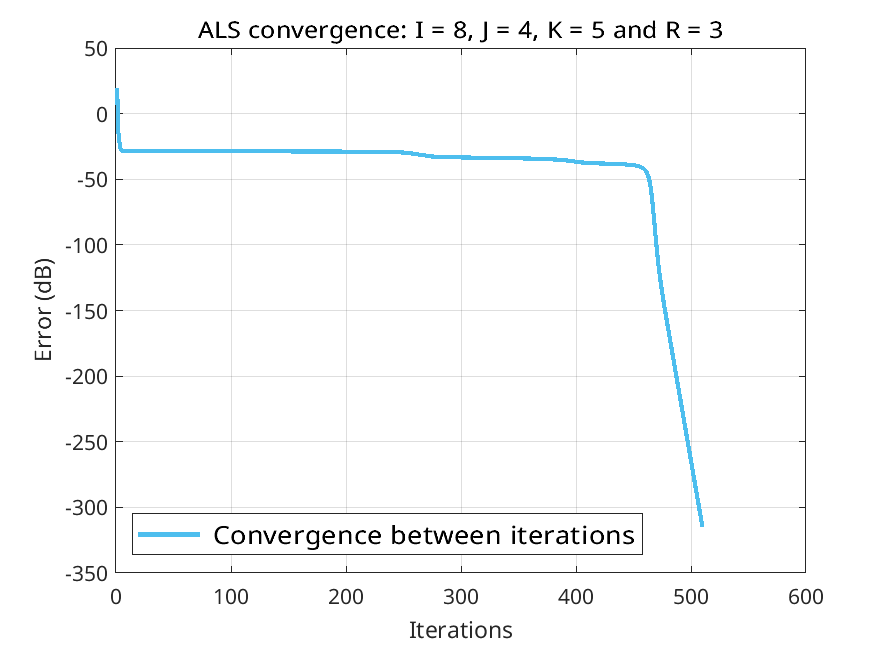
\includegraphics[width=0.75\linewidth]{figs/hw11a1.png} \par 
        \caption{Convergence behavior of ALS algorithm.}
        \label{fig:hw11a1} 
    \end{figure}

    \begin{figure}[ht!]
        \centering 
        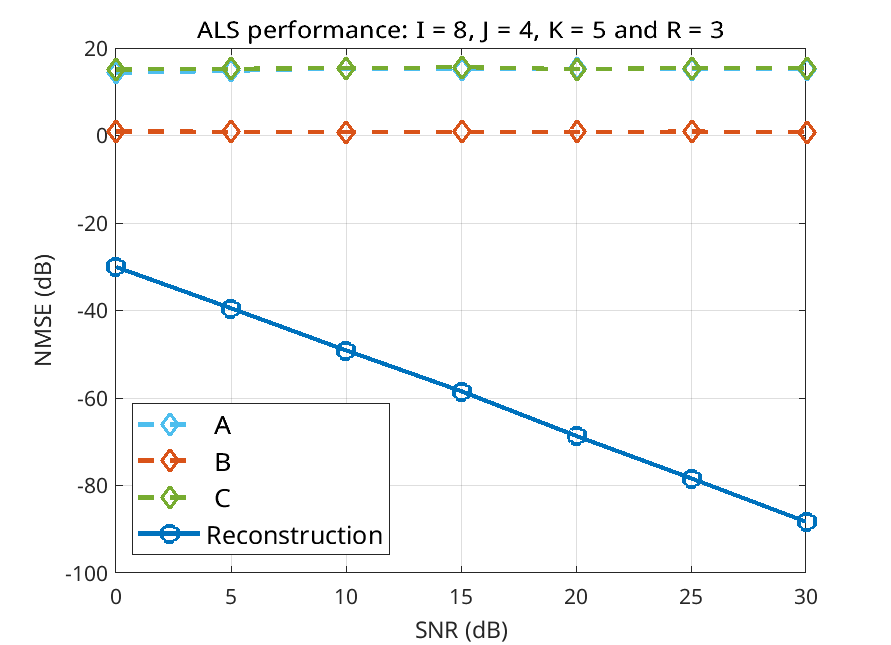
\includegraphics[width=0.75\linewidth]{figs/hw11a2.png} \par 
        \caption{Monter Carlo Experimento with 1000 runs for ALS algorithm.}
        \label{fig:hw11a2} 
    \end{figure}

    \newpage
    \subsection*{Produced Algorithm}

    \begin{verbatim}
        %% Alternate Least-Square (ALS)

        % This function computes the ALS of a given tensor.   
        % Author: Kenneth B. dos A. Benicio <kenneth@gtel.ufc.br>
        % Created: April 2022

        function [Ahat,Bhat,Chat,error] = ALS(X,R)
            I = zeros(R,R,R); 
            for i = 1:R
                I(i,i,i) = 1; 
            end
            [ia,ib,ic] = size(X);

            mode_1 = tensor.unfold(X,1);
            mode_2 = tensor.unfold(X,2);
            mode_3 = tensor.unfold(X,3);

            Ahat = randn(ia,R) + 1j*randn(ia,R);
            Bhat = randn(ib,R) + 1j*randn(ib,R);
            Chat = randn(ic,R) + 1j*randn(ic,R);

            aux = 1000;
            error = zeros(1,aux);
            error(1) = ((norm((mode_1 - Ahat*(tensor.mtx_prod_kr(Chat,Bhat).')),'fro'))^2)/((norm(mode_1,'fro')^2));
            for i = 2:aux
                Bhat = mode_2*pinv((tensor.mtx_prod_kr(Chat,Ahat)).');
                Chat = mode_3*pinv((tensor.mtx_prod_kr(Bhat,Ahat)).');
                Ahat = mode_1*pinv((tensor.mtx_prod_kr(Chat,Bhat)).');
                error(i) = ((norm((mode_1 - Ahat*(tensor.mtx_prod_kr(Chat,Bhat).')),'fro'))^2)/((norm(mode_1,'fro')^2));
                if abs(error(i) - error(i-1)) < eps
                    error = error(1:i);
                    break;
                else
                    continue;
                end
            end
        end

        %% ----- Homework 11 ----- %%
        clc;
        clear;
        close all;

        % Random tensor example
        % I = 8;
        % J = 4;
        % K = 5;
        % R = 3;
        % A = randn(I,R) + 1j*randn(I,R);
        % B = randn(J,R) + 1j*randn(J,R);
        % C = randn(K,R) + 1j*randn(K,R);
        % X = tensor.fold(A*(tensor.mtx_prod_kr(C,B).'),[I J K],1);

        load('homework_11_CPD.mat')
        X = tenX;
        R = 3;

        [ia,ib,ic] = size(X);
        mode_1 = tensor.unfold(X,1);
        mode_2 = tensor.unfold(X,2);
        mode_3 = tensor.unfold(X,3);

        Ahat = randn(ia,R) + 1j*randn(ia,R);
        Bhat = randn(ib,R) + 1j*randn(ib,R);
        Chat = randn(ic,R) + 1j*randn(ic,R);

        aux = 10000;
        error = zeros(1,aux);
        error(1) = ((norm((mode_1 - Ahat*(tensor.mtx_prod_kr(Chat,Bhat).'))...
            ,'fro'))^2)/((norm(mode_1,'fro')^2));
        for i = 2:aux
            Bhat = mode_2*pinv((tensor.mtx_prod_kr(Chat,Ahat)).');
            Chat = mode_3*pinv((tensor.mtx_prod_kr(Bhat,Ahat)).');
            Ahat = mode_1*pinv((tensor.mtx_prod_kr(Chat,Bhat)).');
            error(i) = ((norm((mode_1 - Ahat*(tensor.mtx_prod_kr(Chat,Bhat).'))...
                ,'fro'))^2)/((norm(mode_1,'fro')^2));
            if abs(error(i) - error(i-1)) < eps
                error = error(1:i);
                break;
            else
                continue;
            end
        end

        disp('NMSE (dB) between the original tensor X and its'...
            'reconstruction with MLSKRF:')
        Xhat = tensor.fold(Ahat*(tensor.mtx_prod_kr(Chat,Bhat).'),[ia ib ic],1);
        nmsex = (norm(tensor.unfold(X- Xhat,1),'fro')^2)...
            /(norm(tensor.unfold(X,1),'fro')^2);
        nmsex = 20*log10(nmsex)
        disp('NMSE (dB) between the original matrix A and its estimation:')
        nmsea = (norm(A - Ahat,'fro')^2)/(norm(A,'fro')^2);
        nmsea = 20*log10(nmsea)
        disp('NMSE (dB) between the original matrix B and its estimation:')
        nmseb = (norm(B - Bhat,'fro')^2)/(norm(B,[0.3010 0.7450 0.9330]'fro')^2);
        nmseb = 20*log10(nmseb)
        disp('NMSE (dB) between the original matrix C and its estimation:')
        nmsec = (norm(C - Chat,'fro')^2)/(norm(C,'fro')^2);
        nmsec = 20*log10(nmsec)

        figure
        txt = ['\bf Convergence between iterations'];
        plot(1:i,20*log10(error),'-','color', [0.3010 0.7450 0.9330],...
            "linewidth", 2, "markersize", 8, "DisplayName", txt);
        title(['ALS convergence: I = ' num2str(ia), ', J = ' num2str(ib),...
            ', K = ' num2str(ic), ' and R = ' num2str(R)])
        xlabel('Iterations')
        ylabel('Error (dB)')
        legend_copy = legend("location", "southwest");
        set(legend_copy,'Interpreter','tex','location','southwest',"fontsize", 12)
        grid on;
        saveas(gcf,'hw11a1.png')

        %% ALS in the presence of noisy signals

        I = 8;
        J = 4;
        K = 5;
        R = 3;
        SNR = [0 5 10 15 20 25 30];
        nmse1 = zeros(length(SNR),1);
        nmse2 = zeros(length(SNR),1);
        nmse3 = zeros(length(SNR),1);
        nmse4 = zeros(length(SNR),1);
        for snr = 1:length(SNR)
            for mc = 1:1000
                A = randn(I,R) + 1j*randn(I,R);
                B = randn(J,R) + 1j*randn(J,R);
                C = randn(K,R) + 1j*randn(K,R);
                X = tensor.fold(A*(tensor.mtx_prod_kr(C,B).'),[I J K],1);

                var_noise = 1/(10^(SNR(snr)/10));
                noise = sqrt(var_noise/2)*(randn(I,J,K) + 1j*randn(I,J,K));
                
                X = X + noise;
                
                [ia,ib,ic] = size(X);
                mode_1 = tensor.unfold(X,1);
                mode_2 = tensor.unfold(X,2);
                mode_3 = tensor.unfold(X,3);
                Ahat = randn(ia,R) + 1j*randn(ia,R);
                Bhat = randn(ib,R) + 1j*randn(ib,R);
                Chat = randn(ic,R) + 1j*randn(ic,R);
                aux = 1000;
                error = zeros(1,aux);
                error(1) = ((norm((mode_1 - Ahat*(tensor.mtx_prod_kr(Chat...
                    ,Bhat).')),'fro'))^2)/((norm(mode_1,'fro')^2));
                for i = 2:aux
                    Bhat = mode_2*pinv((tensor.mtx_prod_kr(Chat,Ahat)).');
                    Chat = mode_3*pinv((tensor.mtx_prod_kr(Bhat,Ahat)).');
                    Ahat = mode_1*pinv((tensor.mtx_prod_kr(Chat,Bhat)).');
                    error(i) = ((norm((mode_1 - Ahat*(tensor.mtx_prod_kr(Chat...
                        ,Bhat).')),'fro'))^2)/((norm(mode_1,'fro')^2));
                    if abs(error(i) - error(i-1)) < 1e-6
                        error = error(1:i);
                        break;
                    else
                        continue;
                    end
                end
                Xhat = tensor.fold(Ahat*(tensor.mtx_prod_kr(Chat,Bhat).')...
                    ,[I J K],1);
                
                aux1 = (norm(A- Ahat,'fro')^2)/(norm(A,'fro')^2);
                nmse1(snr,1) = nmse1(snr,1) + 20*log10(aux1);
                aux2 = (norm(B- Bhat,'fro')^2)/(norm(B,'fro')^2);
                nmse2(snr,1) = nmse2(snr,1) + 20*log10(aux2);
                aux3 = (norm(C- Chat,'fro')^2)/(norm(C,'fro')^2);
                nmse3(snr,1) = nmse3(snr,1) + 20*log10(aux3);
                aux4 = (norm(tensor.unfold(X- Xhat,1),'fro')^2)...
                    /(norm(tensor.unfold(X,1),'fro')^2);
                nmse4(snr,1) = nmse4(snr,1) + 20*log10(aux4);
            end
        end
        nmse1  = nmse1/1000;
        nmse2  = nmse2/1000;
        nmse3  = nmse3/1000;
        nmse4  = nmse4/1000;

        figure
        txt = ['\bf A'];
        plot(SNR,nmse1,'--d','color', [0.3010 0.7450 0.9330], "linewidth", 2,...
            "markersize", 8, "DisplayName", txt);
        hold on;
        txt = ['\bf B'];
        plot(SNR,nmse2,'--d','color', [0.8500 0.3250 0.0980], "linewidth", 2,...
            "markersize", 8, "DisplayName", txt);
        hold on;
        txt = ['\bf C'];
        plot(SNR,nmse3,'--d','color', [0.4660 0.6740 0.1880], "linewidth", 2,...
            "markersize", 8, "DisplayName", txt);
        hold on;
        txt = ['Reconstruction'];
        plot(SNR,nmse4,'-o','color', [0 0.4470 0.7410], "linewidth", 2,...
            "markersize", 8, "DisplayName", txt);
        hold off;
        title(['ALS performance: I = ' num2str(I), ', J = ' num2str(J),...
            ', K = ' num2str(K), ' and R = ' num2str(R)])
        xlabel('SNR (dB)')
        ylabel('NMSE (dB)')
        legend_copy = legend("location", "southwest");
        set(legend_copy,'Interpreter','tex','location','southwest',"fontsize", 12)
        grid on;
        saveas(gcf,'hw11a2.png')
    \end{verbatim}
    
\newpage
\section*{Homework 12 \\ Tensor Kronecker Product SVD (TKPSVD)}

    \subsection*{Implementation of TKPSVD}

    \begin{align}
        \mathcal{X} = \sum^{R}_{j = 1} \sigma_{i} \mathcal{A}^{(d)}_{j} \otimes \mathcal{A}^{(d - 1)}_{j}  \otimes \cdots \otimes \mathcal{A}^{(1)}_{j},  
    \end{align}

    \begin{table}[ht!]
        \centering
        \begin{tabular}{|l|l|l|l|}
        \hline
        NMSE($\mathcal{X}, \mathcal{\hat{X}}$) & NMSE($\mathcal{A}^{(1)}, \mathcal{\hat{A}}^{(1)}$) & NMSE($\mathcal{A}^{(2)}, \mathcal{\hat{A}}^{(2)}$) & NMSE($\mathcal{A}^{(3)}, \mathcal{\hat{A}}^{(3)}$) \\ \hline
        -625.5192 & +37.0803 & +0.1706 & +32.5731 \\ \hline
        \end{tabular}
    \end{table}

    \subsection*{Monte Carlo Experiment}

    \begin{figure}[ht!]
        \centering 
        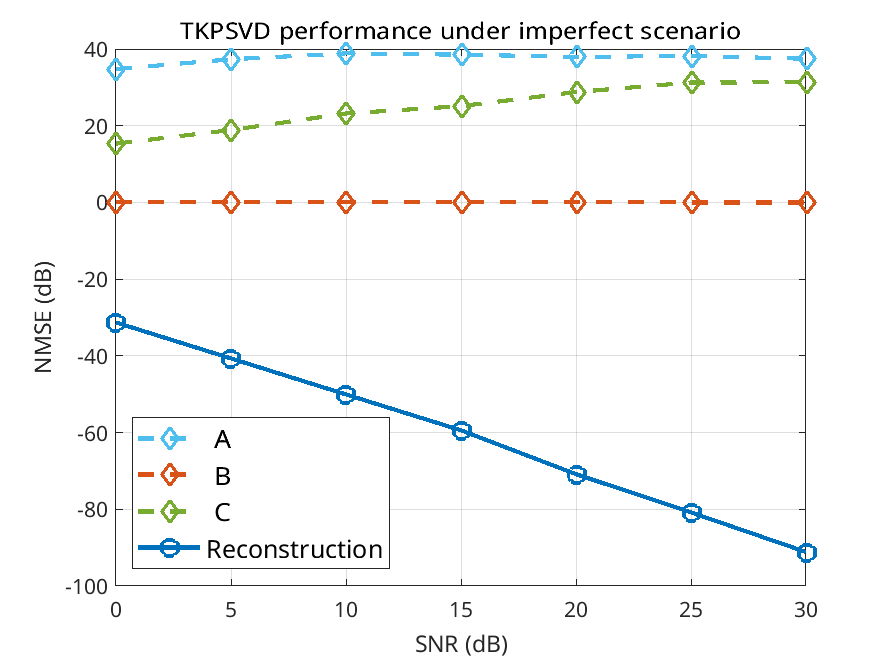
\includegraphics[width=0.75\linewidth]{figs/hw12.png} \par 
        \caption{Monter Carlo Experiment with 1000 runs for TKPSVD algorithm.}
        \label{fig:hw12} 
    \end{figure}

    \newpage
    \subsection*{Produced Algorithm}

    \begin{verbatim}
        %% Tensor Kronecker Product

        % This function computes the Tensor Kronecker Product of two given tensors. 
        % Author: Kenneth B. dos A. Benicio <kenneth@gtel.ufc.br>
        % Created: June 2022

        function C = ten_prod_kron(A,B)
            
            aux1 = num2cell([size(A)]);
            aux2 = num2cell([size(B)]);

            A = repelem(A,aux2{:});
            B = repmat(B,aux1{:});
            C = A.*B;
            
        end

        %% Tensor Kronecker Product Single Value Decomposition (TKPSVD)

        % This function computes the TKPSVD of a tensor.   
        % Author: Kenneth B. dos A. Benicio <kenneth@gtel.ufc.br>
        % Created: June 2022

        function [Ahat,Bhat,Chat] = TKPSVD(tenX,tenSize,tenDim,N,R)
            % First reorder
            var = 1:length(tenSize);
            for n = 1:N
                tenXhatreorder{n} = cell2mat(tenSize(var(n:N:length(tenSize))));
            end
            tenXhatreorder = cell2mat(tenXhatreorder);
            tenXhat = reshape(tenX,tenXhatreorder);
            % Second reorder
            var = 1:length(tenSize);
            for n = 1:N
                tenXhatpermute{n} = var(n:N:length(tenSize));
            end
            tenXhatpermute = cell2mat(tenXhatpermute);
            tenXhat = permute(tenXhat,tenXhatpermute);
            % Third reorder
            tenXhat = reshape(tenXhat,tenDim{:});
            % ALS estimation
            [Ahat,Bhat,Chat,~] = tensor.ALS(tenXhat,R);
        end

        %% ----- Homework 12 ----- %%
        clc;
        clear;
        close all;

        %% TKPSVD 
        R = 1;
        N = 3;

        A = zeros(80,R);
        B = zeros(20,R);
        C = zeros(8,R);
        tenX = zeros(100,16,8);
        for r = 1:R
            tenA = randn(10,4,2);
            %tenA = tenA./frob(tenA);
            A(:,r)= tenA(:);
            tenB = randn(5,2,2);
            %tenB = tenB./frob(tenB);
            B(:,r)= tenB(:);
            tenC = randn(2,2,2);
            %tenC = tenC./frob(tenC);
            C(:,r)= tenC(:);
            varr = tensor.ten_prod_kron(tenC,tenB);
            tenX = tenX + tensor.ten_prod_kron(varr,tenA);
        end

        aux{1} = num2cell(size(tenA));
        aux{2} = num2cell(size(tenB));
        aux{3} = num2cell(size(tenC));
        tenSize = horzcat(aux{:});
        tenDim = cellfun(@(aux) prod(cell2mat(aux)), aux,'UniformOutput',false);

        tenX = tensor.ten_prod_kron(tenC,tenB);
        tenX = tensor.ten_prod_kron(tenX,tenA);

        [Ahat,Bhat,Chat] = tensor.TKPSVD(tenX,tenSize,tenDim,N,R);

        aux1 = aux{1};
        aux2 = aux{2};
        aux3 = aux{3};
        tenXhat = zeros(100,16,8);
        for r = 1:R
            tenAhat_r = reshape(Ahat(:,r),aux1{:});
            %tenAhat_r = tenAhat_r./frob(tenAhat_r);
            tenBhat_r = reshape(Bhat(:,r),aux2{:});
            %tenBhat_r = tenBhat_r./frob(tenBhat_r);
            tenChat_r = reshape(Chat(:,r),aux3{:});
            %tenChat_r = tenChat_r./frob(tenChat_r);
            varr = tensor.ten_prod_kron(tenChat_r,tenBhat_r);
            tenXhat = tenXhat + tensor.ten_prod_kron(varr,tenAhat_r);
        end

        disp('Checking the NMSE (dB) between the original tensor X and its'...
            'reconstruction with TKPSVD:')
        nmsex = (norm(tensor.unfold(tenX- tenXhat,1),'fro')^2)...
            /(norm(tensor.unfold(tenX,1),'fro')^2);
        nmsex = 20*log10(nmsex)
        disp('Checking the NMSE (dB) between the original matrix A and its'...
            'reconstruction with TKPSVD:')
        nmsea = 20*log10((norm(A- Ahat,'fro')^2)/(norm(A,'fro')^2))
        disp('Checking the NMSE (dB) between the original matrix B and its'...
            'reconstruction with TKPSVD:')
        nmseb = 20*log10((norm(B- Bhat,'fro')^2)/(norm(B,'fro')^2))
        disp('Checking the NMSE (dB) between the original matrix C and its'...
            'reconstruction with TKPSVD:')
        nmsec = 20*log10((norm(C- Chat,'fro')^2)/(norm(C,'fro')^2))

        %% Monte Carlo Simulation

        R = 2;
        N = 3;
        SNR = [0 5 10 15 20 25 30];
        nmse1 = zeros(length(SNR),1);
        nmse2 = zeros(length(SNR),1);
        nmse3 = zeros(length(SNR),1);
        nmse4 = zeros(length(SNR),1);
        for snr = 1:length(SNR)
            snr
            for mc = 1:1000
                A = zeros(80,R);
                B = zeros(20,R);
                C = zeros(8,R);
                tenX = zeros(100,16,8);
                for r = 1:R
                    tenA = randn(10,4,2);
                    %tenA = tenA./frob(tenA);
                    A(:,r)= tenA(:);
                    tenB = randn(5,2,2);
                    %tenB = tenB./frob(tenB);
                    B(:,r)= tenB(:);
                    tenC = randn(2,2,2);
                    %tenC = tenC./frob(tenC);
                    C(:,r)= tenC(:);
                    varr = tensor.ten_prod_kron(tenC,tenB);
                    tenX = tenX + tensor.ten_prod_kron(varr,tenA);
                end

                aux{1} = num2cell(size(tenA));
                aux{2} = num2cell(size(tenB));
                aux{3} = num2cell(size(tenC));
                tenSize = horzcat(aux{:});
                tenDim = cellfun(@(aux) prod(cell2mat(aux)), aux,...
                    'UniformOutput',false);

                tenX = tensor.ten_prod_kron(tenC,tenB);
                tenX = tensor.ten_prod_kron(tenX,tenA);
                
                var_noise = 1/(10^(SNR(snr)/10));
                noise = sqrt(var_noise)*(randn(size(tenX)));
                tenX_noisy = tenX + noise;
                
                [Ahat,Bhat,Chat] = tensor.TKPSVD(tenX_noisy,tenSize,tenDim,N,R);

                aux1 = aux{1};
                aux2 = aux{2};
                aux3 = aux{3};
                tenXhat = zeros(100,16,8);
                for r = 1:R
                    tenAhat_r = reshape(Ahat(:,r),aux1{:});
                    %tenAhat_r = tenAhat_r./frob(tenAhat_r);
                    tenBhat_r = reshape(Bhat(:,r),aux2{:});
                    %tenBhat_r = tenBhat_r./frob(tenBhat_r);
                    tenChat_r = reshape(Chat(:,r),aux3{:});
                    %tenChat_r = tenChat_r./frob(tenChat_r);
                    varr = tensor.ten_prod_kron(tenChat_r,tenBhat_r);
                    tenXhat = tenXhat + tensor.ten_prod_kron(varr,tenAhat_r);
                end
                
                var1 = (norm(A - Ahat,'fro')^2)/(norm(A,'fro')^2);
                nmse1(snr,1) = nmse1(snr,1) + 20*log10(var1);
                var2 = (norm(B - Bhat,'fro')^2)/(norm(B,'fro')^2);
                nmse2(snr,1) = nmse2(snr,1) + 20*log10(var2);
                var3 = (norm(C - Chat,'fro')^2)/(norm(C,'fro')^2);
                nmse3(snr,1) = nmse3(snr,1) + 20*log10(var3);
                nmse4(snr,1) = nmse4(snr,1) + 20*log10((norm(tensor.unfold(tenX...
                    - tenXhat,1),'fro')^2)/(norm(tensor.unfold(tenX,1),'fro')^2));
                
            end
        end
        nmse1  = nmse1/1000;
        nmse2  = nmse2/1000;
        nmse3  = nmse3/1000;
        nmse4  = nmse4/1000;

        figure
        txt = ['\bf A'];
        plot(SNR,nmse1,'--d','color', [0.3010 0.7450 0.9330], "linewidth", 2,...
            "markersize", 8, "DisplayName", txt);
        hold on;
        txt = ['\bf B'];
        plot(SNR,nmse2,'--d','color', [0.8500 0.3250 0.0980], "linewidth", 2,...
            "markersize", 8, "DisplayName", txt);
        hold on;
        txt = ['\bf C'];
        plot(SNR,nmse3,'--d','color', [0.4660 0.6740 0.1880], "linewidth", 2,...
            "markersize", 8, "DisplayName", txt);
        hold on;
        txt = ['Reconstruction'];
        plot(SNR,nmse4,'-o','color', [0 0.4470 0.7410], "linewidth", 2,...
            "markersize", 8, "DisplayName", txt);
        hold off;
        title(['TKPSVD performance under imperfect scenario'])
        xlabel('SNR (dB)')
        ylabel('NMSE (dB)')
        legend_copy = legend("location", "southwest");
        set(legend_copy,'Interpreter','tex','location','northeast',"fontsize", 12)
        grid on;
        saveas(gcf,'hw12.png')
    \end{verbatim}
    
\newpage
\section*{Homework 13 \\ Tensor Train Single Value Decomposition (TTSVD)}

    \subsection*{Implementation of TTSVD}
        
    \begin{align}
        \mathcal{X} = \boldsymbol{G}_{1} \bullet^{1}_{2} \mathcal{G}_{2} \bullet^{1}_{3} \mathcal{G}_{3} \bullet^{1}_{4} \boldsymbol{G}_{4},
    \end{align}

    \begin{align}
        \left(\hat{\boldsymbol{G}_{1}}, \hat{\mathcal{G}_{2}}, \hat{\mathcal{G}_{3}}, \hat{\boldsymbol{G}_{4}}\right) = \underset{\boldsymbol{A}, \boldsymbol{B}, \boldsymbol{C}}{\text{min}} \left| \left| \mathcal{X} - \boldsymbol{G}_{1} \bullet^{1}_{2} \mathcal{G}_{2} \bullet^{1}_{3} \mathcal{G}_{3} \bullet^{1}_{4} \boldsymbol{G}_{4} \right| \right|_{\text{F}},
    \end{align}

    \begin{table}[ht!]
        \centering
        \begin{tabular}{|l|l|}
        \hline
        NMSE($\mathcal{X}, \mathcal{\hat{X}}$) with $R = (3,3,3)$ & NMSE($\mathcal{X}, \mathcal{\hat{X}}$) with $R = (2,2,2)$ \\ \hline 
        -606.0326 & -25.1084 \\ \hline
        \end{tabular}
    \end{table}

    \subsection*{Monte Carlo Experiment}

    \begin{figure}[ht!]
        \centering 
        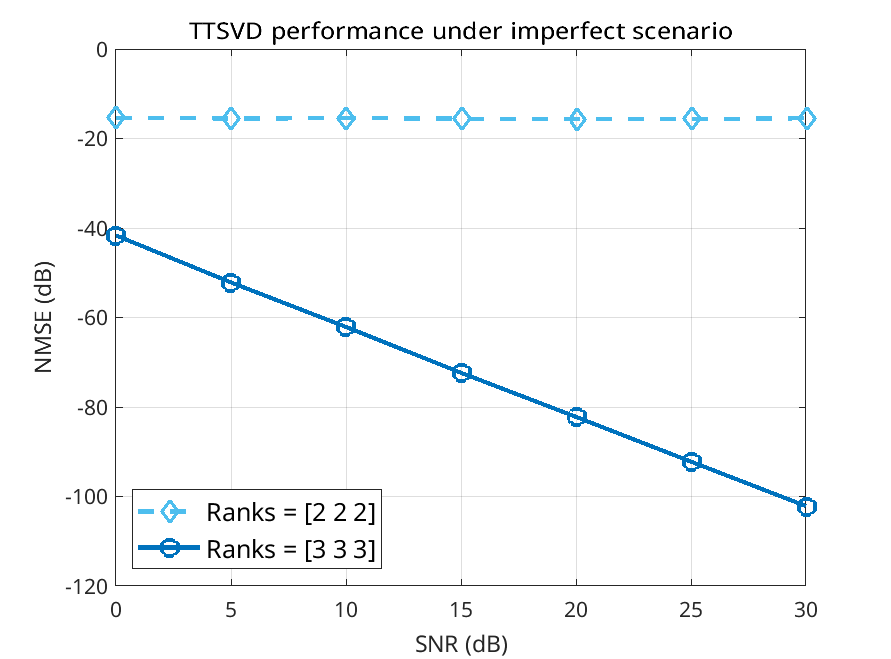
\includegraphics[width=0.75\linewidth]{figs/hw13.png} \par 
        \caption{Monter Carlo Experiment with 1000 runs for TTSVD algorithm.}
        \label{fig:hw13} 
    \end{figure}

    \newpage
    \subsection*{Produced Algorithm}

    \begin{verbatim}
        %% Tensor Contraction

        % This function computes the tensor contraction between a tensor and a matrix
        % or between two tensors.   
        % Author: Kenneth B. dos A. Benicio <kenneth@gtel.ufc.br>
        % Created: June 2022

        function [tenZ] = contraction(tenX,n1,tenY,n2)
            % Obtaining the unfolds
            tenX_n = tensor.unfold(tenX,n1);
            tenY_n = tensor.unfold(tenY,n2);
            % Obtaining the unfold of the contracted tensor
            tenZ_n = (tenX_n.')*tenY_n;
            % Obtaining the fold of the contracted tensor
            dim_x = size(tenX);
            dim_x(n1) = [];
            dim_y = size(tenY);
            dim_y(n2) = [];
            dim_z = [dim_x dim_y];
            tenZ   = tensor.fold(tenZ_n,dim_z,1);
        end

        %% Tensor Train Single Value Decomposition (TT-SVD)

        % This function computes the TT-SVD of a fourth order tensor but can be extended later.   
        % Author: Kenneth B. dos A. Benicio <kenneth@gtel.ufc.br>
        % Created: June 2022

        function [G] = TTSVD(tenX,Ranks)
            X_size = size(tenX);
            % Step 1
            X1 = tensor.unfold(tenX,1);
            [U1,S1,V1] = svd(X1,'econ');
            G1 = U1*sqrt(S1);
            G1 = G1(:,1:Ranks(1));
            G{1} = G1;
            % Step 2
            V1 = sqrt(S1)*V1';
            V1 = V1(1:Ranks(1),:);
            X2 = reshape(V1,[Ranks(1)*X_size(2) X_size(3)*X_size(4)]);
            [U2,S2,V2] = svd(X2,'econ');
            G2 = U2*sqrt(S2);
            G2 = G2(:,1:Ranks(2));
            G{2} = reshape(G2, [Ranks(1) X_size(2) Ranks(2)]);
            % Step 3
            V2 = sqrt(S2)*V2';
            V2 = V2(1:Ranks(2),:);
            X3 = reshape(V2,[Ranks(2)*X_size(3) X_size(4)]);
            [U3,S3,V3] = svd(X3,'econ');
            G3 = U3*sqrt(S3);
            G3 = G3(:,1:Ranks(3));
            G{3} = reshape(G3, [Ranks(2) X_size(3) Ranks(3)]);
            V3 = sqrt(S3)*V3';
            V3 = V3(1:Ranks(3),:);
            G{4} = V3;

            %% ----- Homework 13 ----- %%
        clc;
        clear;
        close all;

        %% Tensor Train SVD for a fourth order tensor
        I1 = 5;
        I2 = 5;
        I3 = 5;
        I4 = 5;
        Ranks = [3 3 3];

        G1 = randn(I1,Ranks(1));
        G2 = randn(Ranks(1),I2,Ranks(2));
        G3 = randn(Ranks(2),I3,Ranks(3));
        G4 = randn(Ranks(3),I4);

        tenX = tensor.contraction(G1,2,G2,1);
        tenX = tensor.contraction(tenX,3,G3,1);
        tenX = tensor.contraction(tenX,4,G4,1);

        [G] = tensor.TTSVD(tenX,Ranks);

        tenXhat = tensor.contraction(G{1},2,G{2},1);
        tenXhat = tensor.contraction(tenXhat,3,G{3},1);
        tenXhat = tensor.contraction(tenXhat,4,G{4},1);

        disp('Checking the TTSVD NMSE (dB) from reconstruction using'... 
            'ranks = [3 3 3]:')
        nmsex = (norm(tensor.unfold(tenX- tenXhat,1),'fro')^2)...
            /(norm(tensor.unfold(tenX,1),'fro')^2);
        nmsex = 20*log10(nmsex)

        Ranks = [2 2 2];
        [G] = tensor.TTSVD(tenX,Ranks);

        tenXhat = tensor.contraction(G{1},2,G{2},1);
        tenXhat = tensor.contraction(tenXhat,3,G{3},1);
        tenXhat = tensor.contraction(tenXhat,4,G{4},1);
        disp('Checking the TTSVD NMSE (dB) from reconstruction using'... 
            'ranks = [2 2 2]:')
        nmsex = (norm(tensor.unfold(tenX- tenXhat,1),'fro')^2)...
            /(norm(tensor.unfold(tenX,1),'fro')^2);
        nmsex = 20*log10(nmsex)

        %% Monte Carlo Simulation
        I1 = 5;
        I2 = 5;
        I3 = 5;
        I4 = 5;
        Ranks  = [3 3 3];
        Ranks1 = [2 2 2];
        Ranks2 = [3 3 3];

        SNR = [0 5 10 15 20 25 30];
        nmse1 = zeros(length(SNR),1);
        nmse2 = zeros(length(SNR),1);
        for snr = 1:length(SNR)
            snr
            for mc = 1:1000
                G1 = randn(I1,Ranks(1));
                G2 = randn(Ranks(1),I2,Ranks(2));
                G3 = randn(Ranks(2),I3,Ranks(3));
                G4 = randn(Ranks(3),I4);

                tenX = tensor.contraction(G1,2,G2,1);
                tenX = tensor.contraction(tenX,3,G3,1);
                tenX = tensor.contraction(tenX,4,G4,1);

                var_noise = 1/(10^(SNR(snr)/10));
                noise = sqrt(var_noise)*(randn(size(tenX)));
                tenX_noisy = tenX + noise;
                
                [GR1] = tensor.TTSVD(tenX_noisy,Ranks1);
                tenXhat = tensor.contraction(GR1{1},2,GR1{2},1);
                tenXhat = tensor.contraction(tenXhat,3,GR1{3},1);
                tenXhat = tensor.contraction(tenXhat,4,GR1{4},1);
                nmse1(snr,1) = nmse1(snr,1) + 20*log10((norm(tensor.unfold(tenX...
                    - tenXhat,1),'fro')^2)/(norm(tensor.unfold(tenX,1),'fro')^2));
                
                [GR2] = tensor.TTSVD(tenX_noisy,Ranks2);
                tenXhat = tensor.contraction(GR2{1},2,GR2{2},1);
                tenXhat = tensor.contraction(tenXhat,3,GR2{3},1);
                tenXhat = tensor.contraction(tenXhat,4,GR2{4},1);
                nmse2(snr,1) = nmse2(snr,1) + 20*log10((norm(tensor.unfold(tenX... 
                    - tenXhat,1),'fro')^2)/(norm(tensor.unfold(tenX,1),'fro')^2));
                
            end
        end
        nmse1  = nmse1/1000;
        nmse2  = nmse2/1000;

        figure
        txt = ['Ranks = [2 2 2]'];
        plot(SNR,nmse1,'--d','color', [0.3010 0.7450 0.9330], "linewidth", 2,...
            "markersize", 8, "DisplayName", txt);
        hold on;
        txt = ['Ranks = [3 3 3]'];
        plot(SNR,nmse2,'-o','color', [0 0.4470 0.7410], "linewidth", 2,...
            "markersize", 8, "DisplayName", txt);
        hold off;
        title(['TTSVD performance under imperfect scenario'])
        xlabel('SNR (dB)')
        ylabel('NMSE (dB)')
        legend_copy = legend("location", "southwest");
        set(legend_copy,'Interpreter','tex',"fontsize", 12)
        grid on;
        saveas(gcf,'hw13.png')
    \end{verbatim}
    
%\bibliographystyle{ieeetr}
%\bibliography{bibliography.bib}

\end{document}